\chapter{Characterising the beam} % (fold)
\label{prt:characterising_the_beam}
\section{Introduction} % (fold)
\label{cha:introduction}
Characterisation of the MuSIC beam was carried out over two years and through a number of experiments. Over the course of two years there were five runs making three significant measurements to characterise the beam: the total charged particle flux; the muon flux (by measuring the muon lifetime); and the muon momentum spectrum. The details of the runs are covered in table~\ref{tab:summary_music_beam_time} along with which experiments were carried out. Several other experiments were also carried out by other groups but these are not discussed here (e.g.\ neutron flux measurements and Mo muon-bombardment experiment).
\begin{table}[htpb]
  \begin{center}
    \begin{tabular}{c|c|c}
      \multicolumn{2}{c|}{Dates}          & Measurements                                \\
      Start            & Stop             &                                             \\
      \hline                                                                             
      29 July 2010     & 31 July 2010     & Charged particle flux.                      \\
      \hline
      \multirow{2}{*}{13 February 2011}
                       & \multirow{2}{*}{16 February 2011}
                                           & Charged particle flux.                     \\
                       &                   & Muon lifetime.                             \\
      \hline
      \multirow{2}{*}{19 July 2011}
                       & \multirow{2}{*}{21 July 2011}
                                          & Muon lifetime.                              \\
                       &                  & Muon yield (via muonic X-rays).             \\
      \hline
      22 October 2011  & 23 October 2011  & Neutron flux.                               \\
      \hline
      \multirow{3}{*}{18 June 2012}
                       & \multirow{3}{*}{22 June 2012}    
                                          & Muon momentum spectrum (via lifetime).      \\
                       &                  & Muon yield (via muonic X-rays).             \\
                       &                  & Mo muon-bombardment.                        \\
    \end{tabular}
  \end{center}
  \caption{A summary of the five MuSIC beam-times with notes on the measurements made.}
  \label{tab:summary_music_beam_time}
\end{table}

This chapter has been split into four sections: the rest of this section will be an introduction to the equipment used for the measurements, with each of the three measurements then treated individually. Each measurement section will cover the set up, the results and analysis of the data.

\subsection{Scintillators Preparation} % (fold)
\label{sub:scintillator_preparation}
As discussed in chapter~\ref{prt:introduction}, scintillating materials produce light when charged particles travel through them. There are several categories of scintillator, those used for our measurements were plastic as they are easy to work with, inexpensive and available in a range of sizes. There are two main considerations in preparing a plastic scintillator: maximising light collection and preventing external light contamination. The standard approach to deal with both of these considerations is to polish and wrap the scintillator.

The scintillator surface is highly vulnerable to damage either through scratches or grease. Damage to the surface of the scintillator is problematic as it inhibits light collected through total internal reflection (TIR). Anything that reduces the amount of TIR increases the amount of light absorbed outside of the scintillator, where it cannot be detected. In order to prevent scratches, scintillators must be handled carefully and protective films are only removed at the last moment. As well as careful handling, the scintillators are cleaned to remove dirt and dust by polishing them with iso-propanol, this removes grease that can also degrade the surface.

Scintillators are generally wrapped with two thin layers: an inner reflective material and an outer blackout material. The inner layer is normally aluminium-mylar or foil, this is wrapped loosely in order to leave a small air gap that has been shown to increase the amount of TIR (and hence light collection). The outer layer is normally a black plastic wrap. This is carefully sealed with tape to prevent light leakage (another aid to this is obviously turning any lights off in the experimental area). An important consideration is to keep the layers as thin as possible in order to minimise energy deposition; to this end overlaps are kept to a minimum.

In order to attach sections of the scintillators together and to attach detectors to the scintillator optical cement and grease were used. Optical cement was used when a permanent fixing was required while grease was used if the components would need to be separated. To use the cement the components were cleaned using iso-propanol, then the two-part glue mixed and applied. A foam jig was used to hold the pieces in place whilst the cement set. When non-permanent joins were required, e.g.\ to attach MPPCs to WLS-fibres, optical grease was used to form the connection. Optical cement and grease have refractive indexes close to (if not the same as) that of the scintillators to maximise transmission either between sections of the scintillator (e.g.\ from the scintillator bulk to the WLS-fibre) or from the scintillator to the MPPC.
% Whilst a significant proportion of scintillator construction is dedicated to increasing reflection back into the scintillator, at the boundary to the MPPC it must be minimised to maximise the amount of light hitting the MPPC (rather than being reflected back into the scintillator).

% subsection scintillator_preparation (end)
\subsection{Multi-Photon Pixel Counters} % (fold)
\label{sub:multi_photon_pixel_counters}
Multi-Photon Pixel Counters (MPPCs, see figure~\ref{fig:images_intro_MPPC_from_hammamatsu_report}) are highly sensitive devices able to accurately count photons over a wide range of intensities. An MPPC is a small device (normally \( \mathcal{O}(1\times1) \)~mm\(^2\)) made from many Avalanche PhotoDiodes (APD) operated in `Geiger-mode'. Each individual APD is a single pixel within the MPPC. The APDs are connected together so that the MPPC's output is the sum of the outputs of the individual pixels. As can be seen in figure~\ref{fig:images_intro_hamamatsu_mppc_waveform_and_counts} there is clear banding that corresponds to the number of incident photons making counts, accurate to the single photon, obtainable when operating within the MPPC's limitations (see below).
\begin{figure}[hptb]
  \centering
    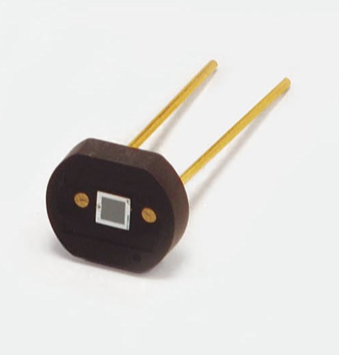
\includegraphics[width=.3\textwidth]{images/intro/MPPC_from_hammamatsu_report.png}
  \caption{Photograph of an MPPC (type S10362-11 with ceramic package) from the Hamamatsu technical report~\cite{hamamatsu_mppc}.}
  \label{fig:images_intro_MPPC_from_hammamatsu_report}
\end{figure}

\begin{figure}[hptb]
  \centering
    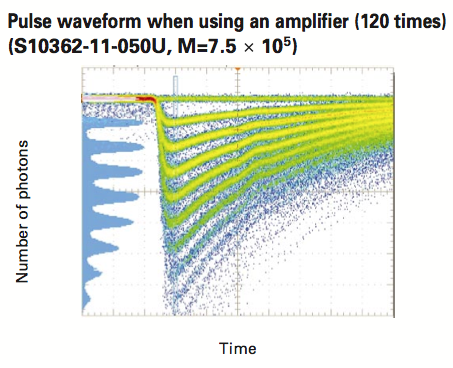
\includegraphics[width=.6\textwidth]{images/intro/hamamatsu_mppc_waveform_and_counts.png}
  \caption{Oscilloscope waveform for an MPPC with a histogram of peak voltage on the left. The histogram shows the clear discrimination between number of photons available on a MPPC. This type of MPPC has \(400\times50\times50 \mu\text{m}^2\) APDs in a \(1\times1\text{mm}^2\) package taken from~\cite{hamamatsu_mppc}.}
  \label{fig:images_intro_hamamatsu_mppc_waveform_and_counts}
\end{figure}

APDs make use of the photoelectric effect and large voltages to produce an `avalanche' of electrons when triggered by an incident photon. A limitation to this system is that an individual APD's output is roughly constant regardless of the number of incident photons. Should the number of photons become comparable to the number of pixels then the MPPC becomes saturated and produces a constant signal as all the pixels fire, rather than clear bands as pixels fire in isolation. For the energy range predicted at MuSIC saturation is not considered to be a significant problem as the number of photons is predicted to be below the one hundred pixels used in our MPPCs (see figure~\ref{fig:sim_n_photons}). 

\begin{figure}[hptb] 
  \centering    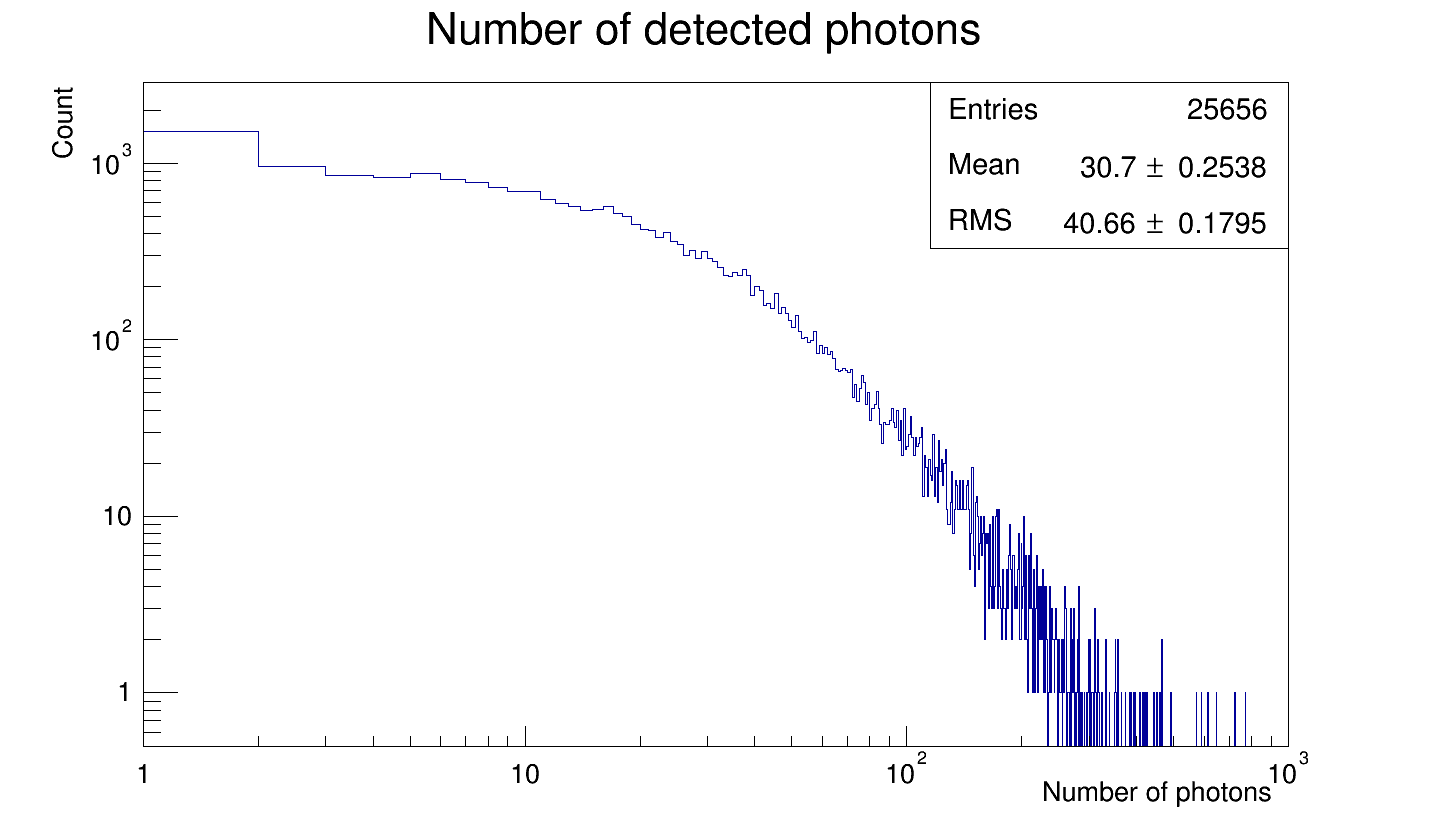
\includegraphics[width=.9\textwidth]{images/plot_generating_scripts/n_photons.png}
  \caption{Simulated distribution of number of photons reaching one of the MPPCs attached, via wavelength shifting fibre, to a \(380\times50\times3.5\)~mm\(^3\) scintillator.}
  \label{fig:sim_n_photons}
\end{figure}


An MPPC has several key attributes: Photon-Detection Efficiency (PDE), peak sensitivity, time resolution, operating voltage (\( V_0 \)), gain (\( M \)) and dark current. The PDE and peak sensitivity respectively describe the likelihood of detection of a photon of given wavelength (see figure~\ref{fig:images_intro_hamamatsu_pde_vs_wavelength}) and the wavelength that the MPPC is most sensitive to (typically \(\sim\)440~nm). Time resolution for MPPCs is generally very good, normally 200--300~ps for FWHM at the single photon level which is more than accurate enough for our purposes. The operating voltage is the potential required to make the MPPC work, due to variance in manufacture this is given individually for each MPPC and has to has to be set correctly for optimum performance, Hamamatsu's MPPCs have \( V_0 = 70\pm10 \)~V. The gain of the MPPC indicates the strength of the signal response to a photon, typical values are between \( 10^5 \) and \( 10^6 \), this corresponds to signals of \( \mathcal{O}(1\text{--}10) \)~\(\mu\)V which must be amplified for accurate measurement. The dark current is a measure of how noisy a particular MPPC is; it is the rate of false signals that have an effective strength equivalent to 0.5~photo-electron (p.e.). Typical values for the dark current are in the range 100--500 kcps (\(\times10^3\)~counts per second) these can be accounted for by correct setting of triggers.
\begin{figure}[hptb]
  \centering
    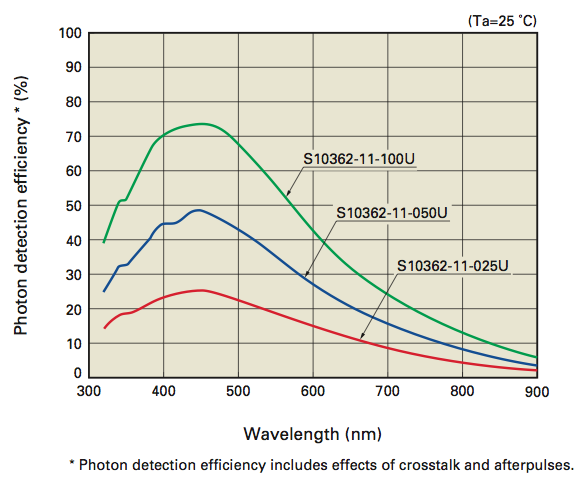
\includegraphics[width=.5\textwidth]{images/intro/hamamatsu_pde_vs_wavelength.png}
  \caption{MPPC Photon Detection Efficiency (PDE) as a function of photon wavelength. A range of pixel densities are shown (100, 400, 1600 pixels/\( 1\times1\text{mm}^2\) for the 100U, 050U and 025U models respectively). Taken from~\cite{hamamatsu_mppc}.}
  \label{fig:images_intro_hamamatsu_pde_vs_wavelength}
\end{figure}

As can be seen, whilst MPPCs have many useful features they do have several features that need careful treatment to make them useful: mainly amplification and noise reduction. These two problems are closely related and in fact, when treated properly one will often help with the other. Given the size of the signal from an MPPC it is obvious that amplification is required to make the signal useable, in fact, as will be discussed below, an unfiltered MPPC signal is too small for detection by most standard equipment. Amplification is done using linear amps which are applied as soon as possible to reduce noise due to cabling as well as attenuation. 
% As well as amplification simple filters are applied to the bias voltage and signal to help reduce noise (see figure~\ref{CIRCUIT DIAGRAM}). Careful ground was also required to reduce noise, this was mainly carried out by ensuring shared ground between different modules.

% subsection multi_photon_pixel_counters (end)
\subsection{Secondary Emission Chamber} % (fold)
\label{sub:secondary_emission_chamber}
As well as studying the resultant beam, knowledge of the initial proton beam is essential for normalisation. This is done using a Secondary Emission Chamber (SEC). A SEC uses thin foils of gold placed within a strong electrical potential. When protons pass through the foils a small number of electrons are produced as part of ionisation, these can then be collected and counted. The SEC only measures a fraction of the beam and even then, only indirectly. In order to calibrate the SEC, runs are performed in which the entire proton beam is absorbed with a copper block downstream of the SEC. Measurement of the total current produced by the block can then be used to determine the fraction absorbed by the SEC, and hence the conversion factor. Measurement of the SEC was carried out using scalers (see below) that counted the cumulative charge passing through the SEC.

% subsection secondary_emission_chamber (end)

\subsection{NIM, CAMAC and VME} % (fold)
\label{sub:nim_and_camac}
Rather than develop custom data acquisition hardware, a modular crate system was used. A crate system supplies power and mechanical fixings for a range of modules, these modules can then be connected together to produce a system. Three crate systems were used: Nuclear Instrument Module (NIM), Computer Automated Measurement And Control (CAMAC) and Versa Module Eurocard bus (VMEbus or VME). NIM supplies power only, whilst CAMAC and VME provide a `backplane' through which data can be transferred to a control card.

NIM modules were primarily used to provide signal processing and data acquisition logic. The CAMAC and VME crates were used for data read-out. Ultimate control and storage was carried out using a PC which recorded the data for later analysis. The rest of this section will discuss the basic modules used in NIM, CAMAC and VME.
\subsection{Discriminators} % (fold)
\label{ssub:discriminators}
A discriminator works by producing a digital signal when an analogue input signal exceeds some preset threshold. Converting the analogue signal to digital makes it much easier to manipulate as many other modules can only use a digital signal. The discriminators were powered by NIM modules and had their thresholds set manually.

Discriminators were used to signal when a certain number of photons were detected by an MPPC i.e.\ when a particle had passed through the scintillator. As the discriminators have a minimum threshold of \(\sim\)25~mV the MPPC signals were amplified to make them useable. As every MPPC has a different gain the thresholds for the discriminators had to be set individually. To normalise between MPPCs the discriminator thresholds were set based on the number of photons the analogue signal corresponded to (see figure~\ref{fig:images_intro_hamamatsu_mppc_waveform_and_counts}). The trigger level (in p.e.)\ was the same for all MPPCs and was chosen to maximise the signal to noise ratio, a typical value was \(\sim2.5\)~p.e.\ which suppressed most of the dark current without compromising sensitivity to charged particles. An oscilloscope could then used to translate the photon (p.e.)\ threshold into a voltage threshold (in mV) that can be used by the discriminator.

% The thresholds had a standard minimum value of \(\sim\)25~mV, in order to meet this linear amplifiers were used to boost the MPPC signal enough to be detectable. 

% subsubsection discriminators (end)
\subsection{Gates and Latches} % (fold)
\label{ssub:gates}
Gates are a set of modules that generally have several related functions. Depending on the mode they can change the length of a signal, delay it, `latch' it or start a clock signal. The first two modes are generally used for creating `gates' (on or off signals) for other modules: e.g.\ turning on a module to record the shape of a signal or indicating to the PC that their is data waiting to be read. A `latch' is a signal that remains on until another signal switches it off, these are often used when it's unclear how long something will take e.g.\ sending data to the PC. Clock signals were generally used as calibration information for other measurements e.g.\ recording the SEC.

% Gates are modules that, when triggered produce an altered signal compared to the input. As well as delaying and lengthening signals gates can also be used in `latch' (or flip-flop) mode. Gates only accept digital signals but can create delays of up to 1~s, and equally change the length by similar amounts. In latch mode the input signal starts the output whilst another input resets it. Latch mode is used to create busy signals by using the input to indicate when the DAQ is processing an event and a signal from the PC to reset it.

% subsubsection gates (end)
\subsection{Logic units} % (fold)
\label{ssub:logic_units}
Logic units provide boolean logic (`AND', `OR', `NOT') for processing digital signals. The limiting factor is the number of inputs that can be combined and the complexity of the combinations. Normally signals are combined in a block with a single module having several discrete blocks. Each block will perform a single logical operation (OR or AND) on its inputs. The inputs of a block can either be normal or negated. A block (or sometimes the entire module) will generally have a veto signal that will stop outputs until the veto is cleared.

Logic units were generally used for simple tests such as checking that all MPPCs on a scintillator had triggered, this helped reduce the number of false positives in addition to the application of a discriminator. Logic units were also used to prevent attempts to process two events at once: if a second event arrived before the previous event was fully processed then the second event was ignored. This leads to `dead time' but is unavoidable.

% subsubsection logic_units (end)
\subsection{Scaler} % (fold)
\label{ssub:scaler}
A scaler is a counting module. It receives a digital input, that when asserted, increments its counter. The most important factor of a scaler is its maximum speed (the maximum input frequency). Events that occur more rapidly than the input frequency will not be properly counted (either not being counted at all or counted as a single event), a typical maximum input frequency is 100~MHz. Most scalers can be daisy-chained together in case their maximum value is exceeded and some allow multiple inputs that can be counted independently. NIM scalers will generally be read-out by eye (e.g.\ using a display) whilst VME/CAMAC modules will be read-out using the crate's data-bus. 

% One of the simplest forms of read out is a count of triggers, this is what a scaler does. The primary concern with a scaler is the input specification to trigger a count as well as the maximum speed at which the unit can count. Modules can either be used with NIM, CAMAC or VME. When the rate is high or the maximum count is low multiple scalers can be daisy-chained together to provide carry over. 

% subsubsection scaler (end)
\subsection{Analogue to Digital Converter} % (fold)
\label{ssub:analogue_to_digital_converter}
There are two primary attributes of an MPPC signal that were measured: its size and its separation from other signals. In order to measure the size of the MPPC signal, an Analogue to Digital Converter (ADC) was used. ADCs work in a variety of ways depending on the exact type of measurement they are making, two common versions used at MuSIC were Peak Sensing ADC (PS-ADC) and Charge-integrating ADCs (QDC). Both types of ADC measure a component of the input analogue signal, the PS type measures the peak voltage whilst the QDC measures the integrated charge, both make these measurements only when enabled by the ADC's `gate'. The ADC's gate is normally set to be slightly longer than the expected signal from an MPPC, i.e.\ \( \sim \)50~ns. 

Several factors define the ADC: the number of bits it is able to read out, the range of input signals that it can measure, its linearity, digitisation/read time (`dead time') and number of channels. The number of bits the ADC has, the range and its linearity work together to determine the accuracy of the ADC; the number of bits determines the resolution between any two values, the range determines the values that the ADC can measure whilst the linearity maps measured values to actual voltages. Dead time measures how long is required to measure the analogue signal and how long it takes to then send the digitised values to the controlling PC i.e.\ for how long the module is inoperative, `dead'. The number of channels on an ADC is a measure of how many inputs it can measure simultaneously, normally one is ascribed to each MPPC so that the triggering signal can be recorded.

A key feature of using an ADC is the pedestal, obviously any analogue signal is going to have some noise that represents its zero level, in an ADC this manifests as a large peak in the lower bins of the ADC, removal of the pedestal is often done by the ADC itself and through the DAQ but it does sometimes have to be removed from the data as well.

% subsubsection analogue_to_digital_converter (end)
\subsection{Time to Digital Converter} % (fold)
\label{ssub:time_to_digital_converter}
A Time to Digital Converter (TDC) measures the time difference between signals. The core parameters for a TDC are the number of bits of precision on each channel, the maximum duration the TDC can record, its linearity, its dead time and number of channels of input. A TDC measures time between a `start' and a `stop' signal. Normally a single start signal is provided to the entire TDC with each channel receiving a stop signal. The measured times between the global start signal and the individual stop signals are then read-out independently. 

An alternative TDC used in later experiments is the Multi-Hit TDC (MH-TDC). Rather than measure a single start/stop pair for each channel the MH-TDC has a ring-buffer to record data for each channel. A ring-buffer has a fixed length (the `window'), typically \(\mathcal{O}(50)\)~\(\mu\)s, when a signal (a `hit') is received its position within the window is marked. The ring-buffer records every hit it receives, regardless of the start signal. When the start signal is received the buffer is read-out, this can be done immediately or after a delay. By using a delay signals both before and after the start signal can be recorded.

 % When the `start' signal is received it signals that the current state of the buffer (and some trailing amount) should be recorded. Using this method, events proceeding the start signal can be recorded as well as those afterwards.

% subsubsection time_to_digital_converter (end)
\subsection{Registers} % (fold)
\label{ssub:registers}
Registers are modules that allow simple logical signals to be sent to or from a PC. In our systems they have two key uses: either indicating to the controlling PC that there is data to be read (an `interrupt') or for the PC to indicate that all the data has been read and that the DAQ should be reset. The interrupt time had to be carefully delayed such that there was long enough for the digitisation to complete whilst minimising dead time. The DAQ reset signal was sent by the PC once it had read all the modules to indicate that data taking could resume.

 % Interrupts were formed using a logic unit and a gate: once a trigger had be formed by the logic unit the gate would delay the interrupt signal long enough for the ADC and TDC digitisation to complete then signal the controlling PC. The PC's reset signal was used to unlatch the veto signals that prevented doubling up of data as well as clear any other latches used by the system.

% Control registers are fairly simple devices but very useful in general control, they act as a simple toggle that can either send or receive a signal to the controlling PC. The main use of registers is to form an interrupt; used this way once data has been taken the ready state of the system can be signalled to the PC and the PC can begin read-out. The interrupt is often delayed so that full digitisation can occur although has to be carefully gauged to prevent excessive dead time. The second common use is to reset the system once read-out has completed, this normally means resetting a latched gate that has been holding the system in veto.

% subsubsection registers (end)
% subsection nim_and_camac (end)
% section experimental_technique (end)
\clearpage
% chapter introduction (end)
\section{Charged Particle Flux} % (fold)
\label{cha:charged_particle_flux}
% TODO Pictures of set ups
% TODO Diagrams of set ups
The first experiment carried out at MuSIC aimed to measure the total flux of charged particles. As well as this measurement it was also a test-bed for the technology and techniques used in later experiments.

Two separate measurements of the charged particle flux were made: one using a long strip scintillator that measured the flux at a range of vertical positions and a second that used a smaller disk that measured the flux at a number of points across the face of the disc.

The DAQ used for these experiments was designed to have a lot greater functionality than was ultimately used. The original design aimed to use the difference of arrival times at the various MPPCs for greater positional accuracy whilst the ADC measurements were intended to measure the energy of the particle; neither of these techniques were successful but the full DAQ is included for completeness.

% These early experiments had DAQ designs that were ultimately superfluous as the data it yielded was not used; this design is included for completeness.
\subsection{Experimental Set Up} % (fold)
\label{sec:experimental_set_up}
The experimental design for both measurements was broadly the same: the scintillators both had four MPPCs attached. In the first measurement a long strip scintillator was used and the MPPCs were distributed evenly across the short ends, for the second measurement the disk had the four MPPCs placed evenly around the circumference (see table~\ref{tab:charged_particle_flux_scint_details}). NIM crates housed the modules for the triggering logic, digitisation was performed via CAMAC modules and the read out data was recorded on a PC to be analysed afterwards. The scintillators were both wrapped with aluminium foil and black wrap and the MPPCs attached via optical cement. The scintillators were mounted on aluminium supports at the end of the beam-pipe.
\begin{table}[hptb]
  \begin{center}
    \begin{tabular}{c|c|c|c}
      Shape  &  Volume (mm\(^3\))           &  MPPCs  &  MPPC positions                    \\
      \hline
      Strip  &  \(380 \times30\times10\)    &  4      &  \( \pm 5 \)~mm on each end.       \\
      Disk   &  \( 35^2\times\pi\times20\)  &  4      &  Radially, every 90\( ^{\circ} \). \\
    \end{tabular}
  \end{center}
  \caption{Details of the scintillators used for the two measurements of the charged particle flux.}
  \label{tab:charged_particle_flux_scint_details}
\end{table}

The aim of these early experiments was to make three measurements: the total trigger rate, the difference in arrival times of light at the MPPCs and the distribution of the number of firing pixels at each MPPC. The total trigger count is proportional to the flux of charged particles through the scintillator. The timing and photon counts were hoped to give information on positioning and the amount of energy deposited but this was found to be incorrect.

% It was hoped that the timing difference between MPPC firings could be correlated to the position of the interaction within the scintillator (this was ultimately incorrect). The distribution of the number of firing pixels was hoped to give some idea of the energy deposited, and possible the types of particles. 

Ultimately only the measurement of the trigger rate was successful. The trigger rate is proportional to the charged particle flux,  assuming negligible dead time. To ensure a negligible dead time, as discussed below, a simplified DAQ system was used and MuSIC was run with a reduced beam current (\(<1\)~nA instead of the MuSIC design current of \(~1\)~\(\mu\)A). Another concern for measuring the charged particle flux are minimally ionising particles (MIPs). MIPs, by definition produce a minimal amount of scintillation light, making their detection difficult. The thickness of the scintillators, especially the second (20~mm) should still be sensitive to MIPs.

% to mitigate this a thicker scintillator (20~mm) was used for the second measurement in which more energy would be deposited.

The DAQ used to measure the trigger rate was a subset of the full DAQ, used to measure the time and energy:
\begin{enumerate}
  \item Amplify the MPPC signal to a detectable level.
  \item Remove dark current using a discriminator.
  \item Create a trigger and veto from the coincidence of all MPPCs: an `AND' operation applied to the output of the discriminators.
   % logic module to form a trigger (further removing noise) and raise a veto based on the coincidence of events from all MPPCs.
  \item Record the analogue MPPC signal using an ADC.
  \item Use the trigger and the first MPPC's signal to start the TDC.
  \item Delay three of the remaining signals to form the stops to the TDC (the delay can be removed to regain the accurate time).
  \item Remove the veto on the system once read-out is complete.
\end{enumerate}
This can be seen as a schematic in figure~\ref{fig:MuSIC1_DAQ_Block}. 

\begin{figure}[hptb]
  \centering
  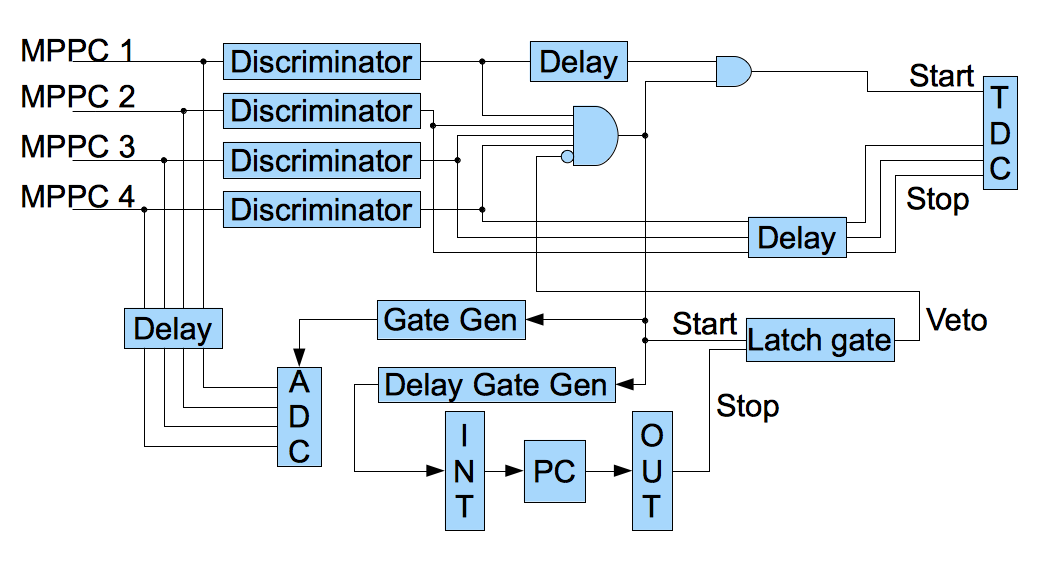
\includegraphics[width=.9\textwidth]{images/charged_flux/MuSIC1_DAQ_Block.png}
  \caption{Schematic of the DAQ used for measuring the charged particle flux. Horizontal blocks indicate NIM units whilst vertical units were mounted in a CAMAC crate. The two `AND' blocks were made using NIM modules.}
  \label{fig:MuSIC1_DAQ_Block}
\end{figure}

To make the final measurement of the trigger rate, the majority of the DAQ was ignored and the four-fold coincidence counted using a scaler. By counting the raw triggers, effects of dead time could be negated and a truer value for the number of interactions obtained. For the 1D experiment, measurements were made over 50~s with control done via hand, this obviously had limitations 

The positions of the two experiments are given in table~\ref{tab:flux_setup} with respect to the centre of the beam-pipe. `By-eye' read-out of the 1D measurement was done using a display mounted on the scaler used to count triggers. For the 2D measurement a CAMAC module was used that was read out by computer. It's important to note that not only were the detectors very different but due to experimental constraints the 2D measurement was made significantly further from the end of the beam pipe than the 1D experiment (85~cm compared to 6~cm).
\begin{table}
  \begin{center}
    \begin{tabular}{c|c|c|c|c|c}
      Measurement  &  \multicolumn{3}{c|}{Distance from centre of beam (cm)}         &  Scaler    &  Read-scout \\
      &    Horizontal    &       Vertical              &  Longitudinal  &  Time (s)  &          \\
      \hline            
      1D           &  0               &  \(-5\), \(-15\), 0, 15, 5  &       6        &  50        & By-eye   \\
      2D           &  \(-17\), 0, 17  &  \(-16\), 0, 20, 25         &       85       &  20        & CAMAC    \\
    \end{tabular}
  \end{center}
  \caption{Positions at which the charged particle flux was measured, 1D refers to the first run in which only the vertical displacement was measured, 2D refers to the second run in which horizontal measurements were also take. The distances from the beam-pipe were 6~cm for 1D measurements and 85~cm for 2D, this was due to mechanical constraints.}
  \label{tab:flux_setup}
\end{table}

% section experimental_set_up (end) 
\subsection{Detector efficiency} % (fold)
\label{sec:detector_efficiency}
As well as making measurements of the charged particle flux another important measurement, made soon after the second beam time, was measurement of the efficiency of the circular detector. This was done using three large (\( 40\times40\times1 \)~cm\(^3\)) scintillator paddles. Light from the scintillators was detected using Photo-Multiplier Tubes (PMT). The three large paddles were positioned sandwiching the circular scintillator, two above and one below. 

The circular detector's efficiency was calculated using the ratio of detections by the PMTs to detection by the MPPCs (once size considerations had been taken into account). It was assumed that the rate of detection by the circular scintillator was proportional to the detection rate in the three large scintillators. The first test was the efficiency of all three remaining MPPCs (one had become irrevocably damaged during beam time) then the efficiency of pairs of MPPCs was tested. Testing consisted of counting the occurrence of three-fold coincidence on the PMTs and either two or three fold coincidence on the MPPCs. Data was taken for approximately one day for each configuration. The MPPCs were not tested individually to ensure that dark current events were not included, although these were reduced by using a discriminator to produce the signals. The results of this measurement are shown in table~\ref{tab:music2_eff}.

\begin{table}
  \begin{center}
    \begin{tabular}{c | c | c | c | c | r@{~\( \pm \)~}l}
      \multirow{2}{*}{Configuration} 
                     &  Run Time             &  MPPC   &  PMT        &  \multirow{2}{*}{Efficiency} 
                                                                                    &  \multicolumn{2}{c}{Adjusted}   \\
                     &  (\(\times 10^3\)~s)  &  Count  &  Count      &              &  \multicolumn{2}{c}{Efficiency} \\
      \hline
      123            &  86.0                 &  1651   &  1,161,165  &  0.00142     &  0.0591 & 0.0015  \\
      12             &  92.3                 &  6055   &  1,229,389  &  0.00493     &  0.2048 & 0.0026  \\
      13             &  87.1                 &  5653   &  1,179,116  &  0.00479     &  0.1993 & 0.0027  \\
      23             &  84.4                 &  3999   &  1,129,137  &  0.00354     &  0.1472 & 0.0023  \\
        
    \end{tabular}
  \end{center}
  \caption{Summary of the data taken for measuring the MPPC detector efficiency. Configuration refers to which of the three MPPCs were tested. The efficiency is the simple ratio of the MPPC count to the PMT count whilst the adjusted efficiency has been scaled by the ratio of the areas of the scintillators, i.e.\ by \( \frac{40\times40}{\pi3.5^2} \).}
  \label{tab:music2_eff}
\end{table}

Assuming that the total efficiency (\( \epsilon_t \)) is the product of the individual efficiencies (\( \epsilon_{1,2,3} \)) then it can be expressed as:
\begin{align}
  \epsilon_t &= \epsilon_1  \epsilon_2  \epsilon_3
\end{align}
With the measured efficiencies of the pairs of MPPCs we can calculate the individual efficiencies by solving:
\begin{align*}
  \epsilon_{12} &= \epsilon_{1} \epsilon_{2} &\implies   \epsilon_{1}  &= \frac{\epsilon_{12}}{\epsilon_{2}}                       \\
  \epsilon_{13} &= \epsilon_{1} \epsilon_{3} &\implies   \epsilon_{2}  &= \frac{\epsilon_{12}\epsilon_{3}}{\epsilon_{13}}          \\
  \epsilon_{23} &= \epsilon_{2} \epsilon_{3} &\implies   \epsilon_{3}  &= \sqrt{\frac{\epsilon_{23}\epsilon_{13}}{\epsilon_{12}}}  \\
\end{align*} 
This can be generalised to:
\begin{align*}
  \epsilon_{i} &= \sqrt{\frac{\epsilon_{ij}\epsilon_{ik}}{\epsilon_{jk}}} \label{equ:individual_eff}
\end{align*}
Where \( \epsilon_i \) is a single efficiency we want to calculate and \( \epsilon_{jk} \) is the combined measurement of the other two efficiencies. Applying this to table~\ref{tab:music2_eff} we get the efficiencies for the MPPCs shown in table~\ref{tab:calculated_individual_eff}. It's important to note that these efficiencies represent more than just the individual MPPC's quantum efficiency but the entire gestalt of systematic effects that contribute to the efficiency of the specific MPPC including scintillator acceptance (both geometric and energetic), light collection and transmission. As can be seen the estimated total efficiency ends up being larger than what was actually measured but this is to be expected as the system assumes all the efficiencies are completely independent of one another. Using these values the average efficiency of a single MPPC can be calculated and given an error as seen in the final line of the table.

\begin{table}
  \lineup
  \begin{center}
    \begin{tabular}{c|r@{~\(\pm\)~}l}
      MPPC  &  \multicolumn{2}{c}{Efficiency} \\
      \hline
      1  &  0.5265 & 0.0064  \\
      3  &  0.3786 & 0.0046  \\
      2  &  0.3889 & 0.0048  \\
      \hline
      \( 123_{Calc} \)  &  0.0775  &  0.0016  \\
      \( 123_{Meas} \)  &  0.0591  &  0.0015  \\
      \hline 
      \( \epsilon_{\text{Ave.}} \)  &  0.431\0 & 0.067 \\
         
    \end{tabular}
  \end{center}
  \caption{Efficiencies of individual MPPCs calculated using the values from table~\ref{tab:music2_eff}, and equation~\eqref{equ:individual_eff}. The two values below the line represent the total efficiency as calculated using the individual values and the measured value. The final value, \(\epsilon_{\text{Ave.}}\) is the mean efficiency of the three individual efficiencies, it's error is the standard deviation of those values. Note: these values include any acceptance effects, the light collection efficiencies of the scintillator and any effects due to the DAQ.}
  \label{tab:calculated_individual_eff}
\end{table}


% section detector_efficiency (end)
\subsection{Results} % (fold)
\label{sec:results}

Prior to the main experiments the conversion factors from SEC count to proton current was determined, these values were determined to be, respectively for the 1D and 2D measurement: 0.03408~nA and 1.514~nA. The results from the measurements are presented in table~\ref{tab:1d_res}, for the 1D case, and table~\ref{tab:2d_res} in the 2D case. The counts were converted to rates and the flux calculated using:
\begin{align}
  j &= \frac{F(C - C_{off})}{I_{p}} \\
  I_{p} &= K(S - S_{off})
\end{align}
where \(j\) is the flux, \(F\) is a scaling factor, \(C\) is the trigger count with the beam on, \(C_{off}\) is the background trigger rate (i.e.\ with the beam off), \( I_{p} \) is the proton current, \(S\) is the SEC count, \(S_{off}\) is the SEC count with the beam off and \(K\) is the SEC to current conversion factor. The scaling factor, \(F\), was used to account for different conditions between runs. \(F\) was taken to be the ratio of the measurements made at the same location. I.e.\ the scaling factor for the 1D case was the ratio of the two measurements made at 0~cm. For the 1D measurement there was a difference between the first four and last five measurements due to damage to the MPPCs (one broke and another became detached from the scintillator). The 2D measurements were made at a larger distance than the 1D measurements as there was another experiment upstream that prevented closer positioning. The upstream experiment was used to make the muon lifetime measurement discussed below, it consisted of two scintillators on either side of stopping target. The stopping target was initially 20~mm of magnesium that was changed to 5~mm of copper for the final 3 runs.


\begin{table}
  \begin{center}
    \begin{tabular}{ r | r | c | c | c | c | r@{~\(\pm\)~}r } 
      Height   &  \multicolumn{2}{c|}{Trigger Count}    &  \multicolumn{2}{c|}{SEC Count}  &  Factor   &  \multicolumn{2}{c}{Flux (\(j\))}          \\
      (cm)     &  \multicolumn{1}{c|}{(\(C\))}  
                             &  (\(C_{off}\))           &    (\(S\))   &   (\(S_{off}\))   &  (\(F\))  &  \multicolumn{2}{c}{(nA\(^{-1}\))} \\
      \hline
        0      &  2,151,736  &    \multirow{4}{*}{30}   &   1,255  &  \multirow{4}{*}{381} &  \multirow{4}{*}{\(1.0\pm0.0\)}  
                                                                                                      &  72,200 & 3,300  \\
      \(-5 \)  &  1,438,685  &                          &   1,286  &                       &          &  46,600 & 2,100  \\
      \(-15\)  &    446,302  &                          &   1,212  &                       &          &  15,770 &   760  \\
      \(-15\)  &    502,596  &                          &   1,208  &                       &          &  17,830 &   860  \\
      \hline            
        5      &  1,663,702  &   \multirow{4}{*}{83}    &   1,298  &  \multirow{4}{*}{398} &  \multirow{4}{*}{\(1.684\pm0.034\)}  
                                                                                                      &  91,300 & 4,000  \\
        5      &  1,420,836  &                          &   1,142  &                       &          &  94,300 & 4,800  \\
       15      &  1,080,170  &                          &   1,336  &                       &          &  56,900 & 2,400  \\
       15      &  1,185,051  &                          &   1,371  &                       &          &  60,200 & 2,500  \\    
       \hline
        0      &  1,307,015  &         34               &   1,298  &             404       & \(1.684\pm0.078\)
                                                                                                      &  72,200 & 3,200  \\
    \end{tabular}
  \end{center}
  \caption{Summary of the results from the measurement of the vertical charged particle flux. The errors are statistical whilst the error on \(F\) is calculated as the errors on the un-scaled measurements at 0~cm added in quadrature. The error on the flux is calculated as the propagated errors of the other values. Counts were taken for 50~s. The SEC conversion factor, \(K\), was 0.03408~nA. The factor was taken to be the ratio of two measurements made at 0~cm. The 0~cm measurements were used as this was the only pair of measurements that were made with the experiment in both conditions (i.e.\ all MPPCs functional and later, with one broken and another damaged).}
  \label{tab:1d_res}
\end{table}


\begin{figure}[hptb]
  \centering
  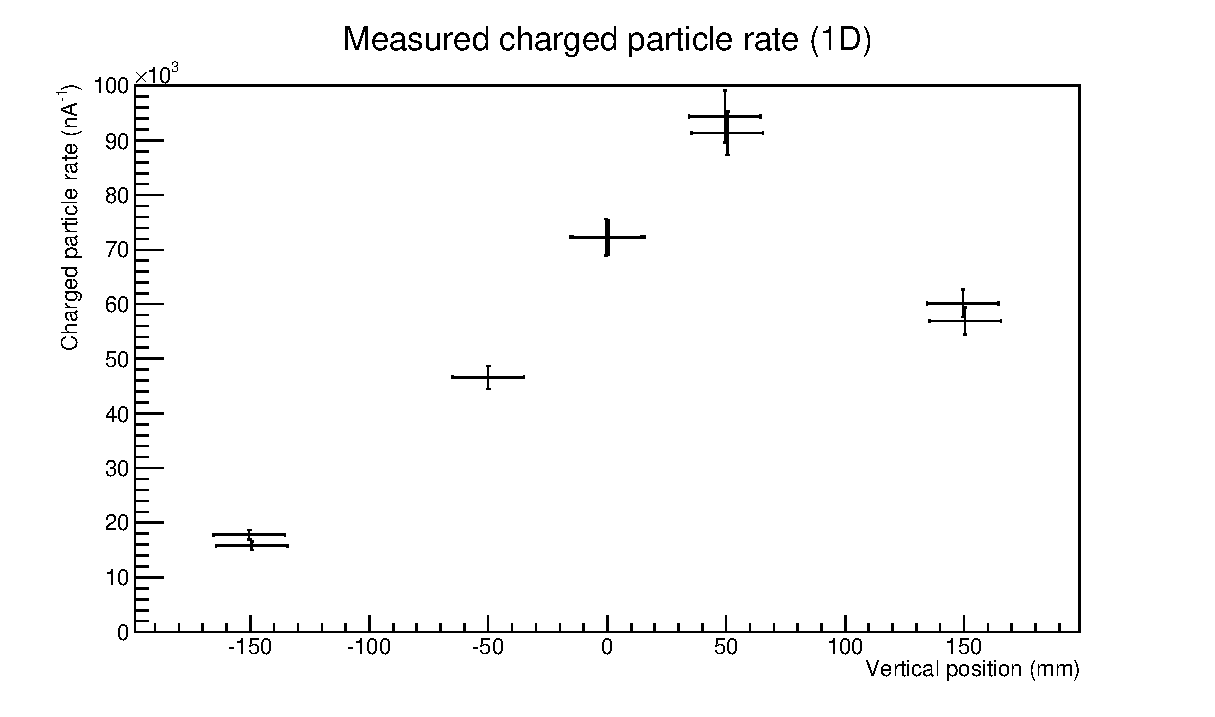
\includegraphics[width=.8\textwidth]{images/plot_generating_scripts/measured_1d_charged_flux.eps}
  \caption{Measurement of the 1D charged particle flux as given in table~\ref{tab:1d_res}. Where two measurements were made at a single location an offset has been applied to the point to allow clearer reading of the plot, the measurements were actually at the same position. The errors on the vertical position are the width of the scintillator used.}
  \label{fig:images_hit_rate_rescaled}
\end{figure}


% Values calculated in https://docs.google.com/spreadsheet/ccc?key=0Ahpo2ep0Rqg5dGNBZk9EZTZmc2w1N0RiR2UwSHZkQ0E#gid=4
% and get_average_hit_rates used to calculate the rates
\begin{table}
  \begin{center}
    \begin{tabular}{r | r | r | c | c | c | r@{~\(\pm\)~}r | r@{~\(\pm\)~}r}
      \multicolumn{1}{c|}{X}     &   \multicolumn{1}{c|}{Y}    &  \multicolumn{2}{c|}{Trigger Count}  &  \multicolumn{1}{c|}{SEC Count}  &  \multicolumn{1}{c|}{Factor}  &  \multicolumn{2}{c|}{Flux (\(j\))}  &  \multicolumn{2}{c}{Simulated (\(j\))}\\
      \multicolumn{1}{c|}{(cm)}  &  \multicolumn{1}{c|}{(cm)}  &         \multicolumn{1}{c|}{(\(C\))}  &  \multicolumn{1}{c|}{(\(C_{off}\))}         &  \multicolumn{1}{c|}{(\(S\))}    &   (\(F\))  &  \multicolumn{2}{c|}{(nA\(^{-1}\))}  &  \multicolumn{2}{c}{(nA\(^{-1}\))}   \\
      \hline
        0      &    0      &           68,761 & 58                &   51        &  \multirow{2}{*}{\(1.0\pm0.0\)}
                                                                                           &   5,400  &  1,000  &   4,287 & 65 \\
      \(-17\)  &   20      &          117,947 & 58                &   51        &          &   9,300  &  1,700  &   1,347 & 37 \\
      \hline
      \(-17\)  &  \(-16\)  &           39,528 & 48                &   68        & \multirow{8}{*}{\(1.0\pm0.0\)}  
                                                                                           &   2,210  &   330  &     492 &  22 \\
      \(-17\)  &    0      &           97,190 & 78                &   73        &          &   5,010  &   710  &   6,952 &  83 \\
       17      &    0      &           63,160 & 91                &   76        &          &   3,110  &   430  &   1,174 &  34 \\
       17      &   20      &          105,097 & 88                &   71        &          &   5,590  &   810  &     902 &  30 \\
       17      &  \(-16\)  &           27,010 & 55                &   67        &          &   1,540  &   230  &     975 &  31 \\
        0      &  \(-16\)  &           43,634 & 97                &   69        &          &   2,400  &   360  &   1,752 &  42 \\
        0      &   20      &          142,536 & 73                &   64        &          &   8,600  & 1,300  &  11,160 & 110 \\
        0      &    0      &           75,376 & 60                &   66        &          &   4,360  &   670  &   4,287 &  65 \\
      \hline
         0      &   25     &           45,950 & 35                &   46        &   \multirow{3}{*}{\(1.65\pm0.37\)}
                                                                                           &   6,800  &  2,100  &  1,216 &  35 \\
       \(-17\)  &   25     &           69,582 & 119               &   47        &          &  10,000  &  3,000  &    914 &  30 \\
         0      &   20     &           80,088 & 238               &   60        &          &   8,600  &  2,400  & 11,157 & 106 \\
    \end{tabular}
  \end{center}
  \caption{Table of the results from the 2D measurement. The trigger count measurements were made over 20~s apart from the first two measurements of the trigger count with the beam off which were made over 11~s. The SEC measurements were made over 100~s. Counts were made using a CAMAC controlled scaler and an enable gate triggered via interrupt register. The column for the SEC bias, \(S_{off}\), is elided as it was constant at 9 and the SEC conversion factor, \(K\), was 1.514~nA. As with the 1D measurement the errors are statistical. The last three values also include an error due to the calculation of the scaling factor.}
  \label{tab:2d_res}
\end{table}
 
\begin{figure}[hptb]
  \centering
  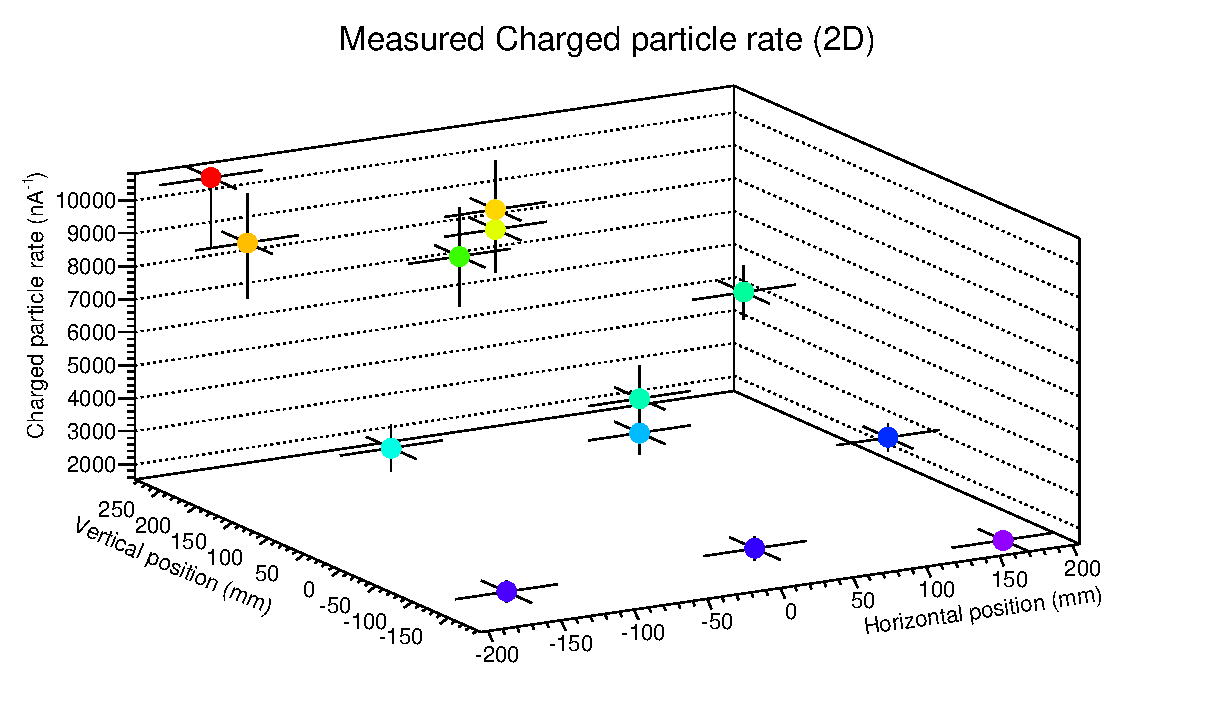
\includegraphics[width=.8\textwidth]{images/plot_generating_scripts/measured_2d_charged_flux.eps}
  \caption{2D plot of the charged particle flux across the front of the MuSIC beam pipe. The final three measurements were rescaled using the ratio of the two measurements at \((0,20)\)~cm.}
  \label{fig:2D_flux}
\end{figure}
 
% section results (end)
\subsection{Analysis} % (fold)
\label{sec:analysis}
As can be seen from the figures~\ref{fig:images_hit_rate_rescaled}~and~\ref{fig:2D_flux} the beam spot is positioned slightly up and to the left of the centre of the pipe. Where there were multiple measurements at the same position there is good agreement which suggests that the measurements are correct.

The agreement between the measurements and the simulation is less good as shown by figure~\ref{fig:images_plot_generating_scripts_1D_charged_particle_flux} where clearly the simulated rate and the measured rate are off by a significant amount (although both have the same shape). Comparing the simulation of the 2D case (figure~\ref{fig:sim_2d_charged_flux}) with the measurement (figure~\ref{fig:2D_flux}) we see that the simulation predicts a much more intense beam spot than what we see. This is likely due to the G4BL simulation having a much simpler model of the magnetic field at the position of the 2D measurement. The fluxes (with the exception of the peak at (0~cm, 20~cm)) are lower in the simulation than measured but not to the same degree as in the 1D case.

As figure~\ref{fig:sim_2d_charged_flux} shows both measurements agree on the general position of the beam spot. The measurements are not directly comparable due to the differences in both scintillator volume and position with respect to the end of the beam-pipe. Obviously the flux for the 2D measurement is generally lower due to smaller scintillator and greater distance from the beam-pipe.

The detector efficiency measurement for the 2D apparatus allows a more accurate calculation of the flux for this case whilst also providing a bench-mark efficiency for future uses of the scintillator/MPPC configuration (where it wasn't always possible to make an analogous measurement). 

The biggest problem, and one which was a cause of many issues, was the fragility of the MPPCs. Both the MPPC itself and the optical cement that bonded them to the scintillator were liable to break and this caused many problems that could not be easily fixed during the time available. 

A significant issue with the 1D measurement is the lack of a confirmation measurement that allows verification of the scaling factor applied to the later results. Even if the re-scaled points are ignored then they confirm that the beam spot is in the upper half of the pipe, a measurement later confirmed by the 2D measurement. 

Comparing the measured and simulated rates yields some interesting features. There is broad agreement on the general shape of the distribution but, using normalised plots, it appears that the measured charged particle rate for the 1D measurement is consistently higher than the simulated value by a factor of between 2 and 10. No obvious explanation of this presents itself as the measured value, should be, a lower bound whilst the simulated value should be closer to the `true' value due to lack of detector affects and similar. Whilst this suggests that further development of the G4BL simulation is required it is encouraging that MuSIC is performing above expectations, it also indicates that with improved experiments these sorts of measurements should provide useful data for tuning these models.

% \begin{figure}[hptb] 
%   \centering
%     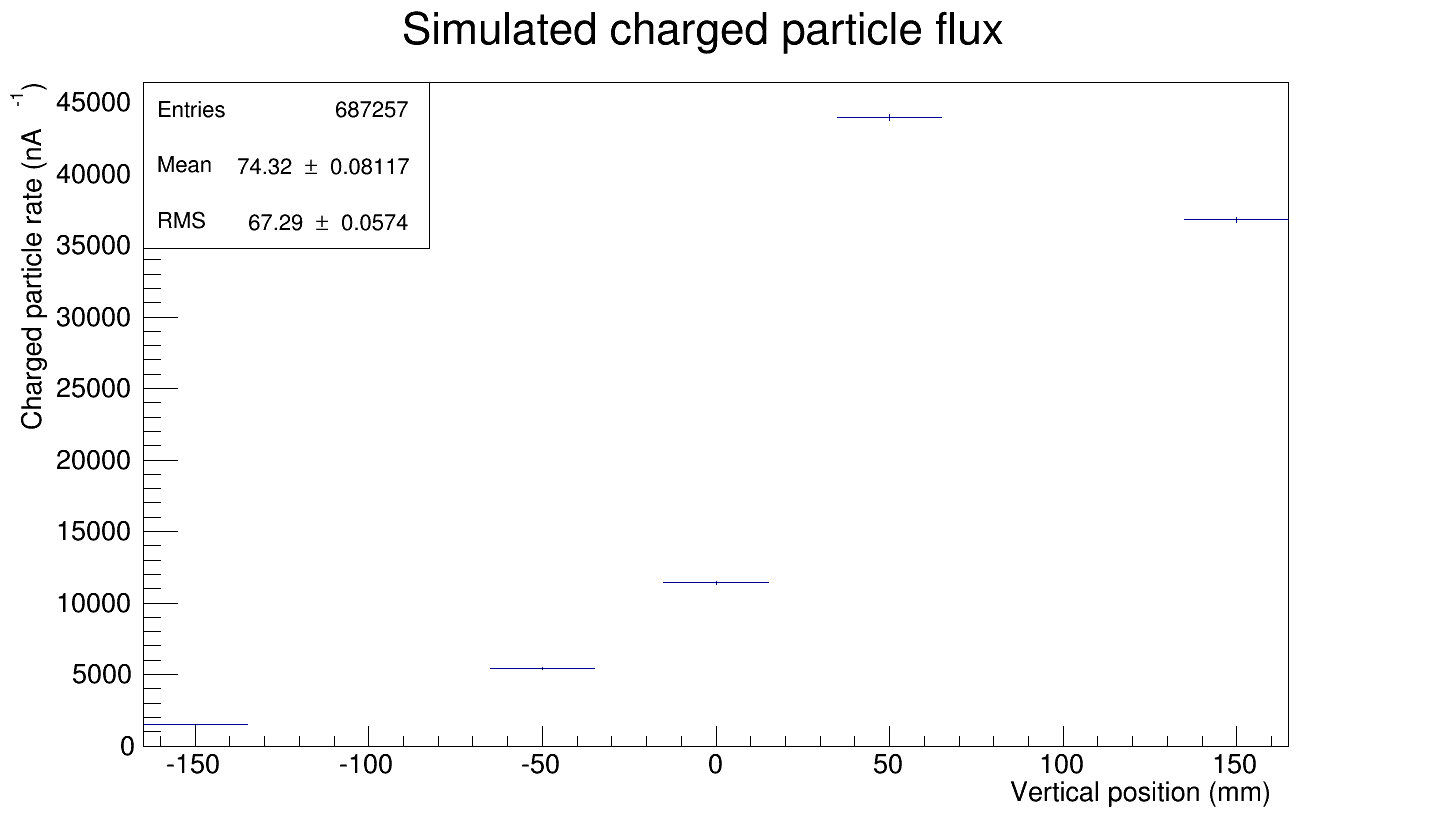
\includegraphics[width=.9\textwidth]{images/plot_generating_scripts/sim_1d_charged_flux.png}
%   \caption{Simulated results for the 1D charged particle rate, normalised to a proton current of 1~nA. Values calculated as the un-adjusted number of charged particles in the 1D scintillator volume from \( 9\times10^8 \) initial protons generated in G4BL.}
%   \label{fig:sim_1d_charged_flux}
% \end{figure}
\begin{figure}[hptb]
  \centering
    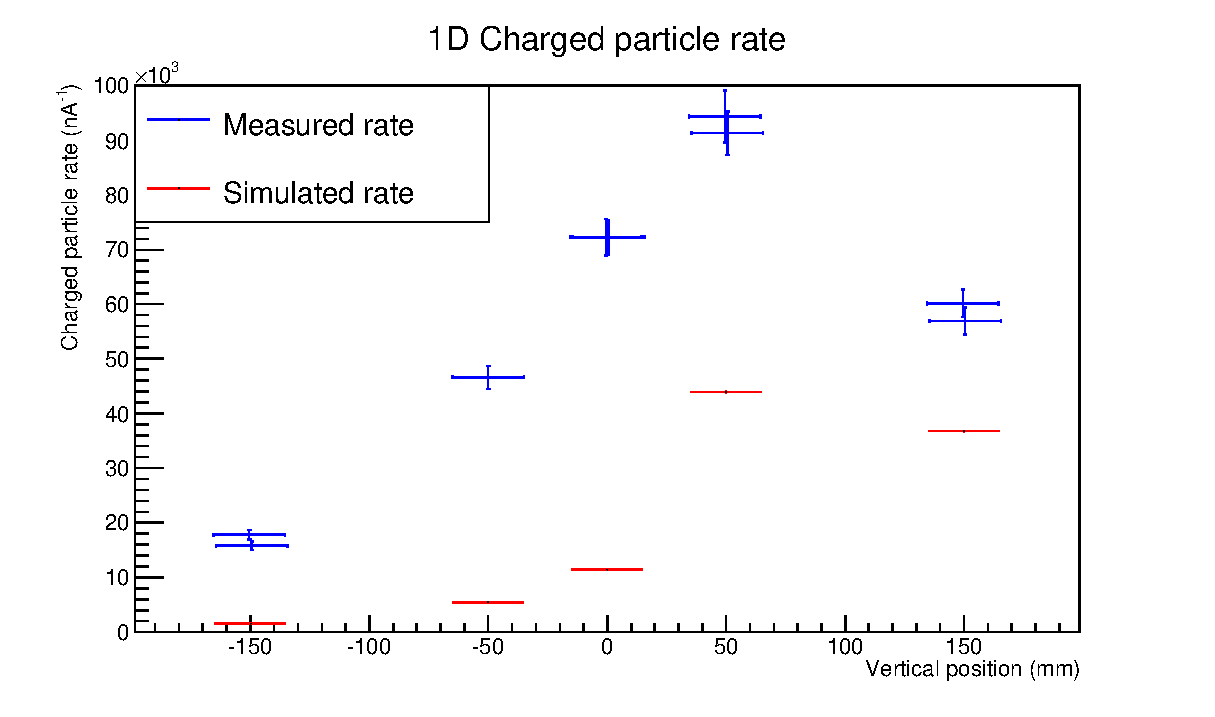
\includegraphics[width=.9\textwidth]{images/plot_generating_scripts/1D_charged_particle_flux.eps}
  \caption{Comparison of simulated and measured total charged particle flux.}
  \label{fig:images_plot_generating_scripts_1D_charged_particle_flux}
\end{figure}
  
\begin{figure}[hptb]
  \centering  
    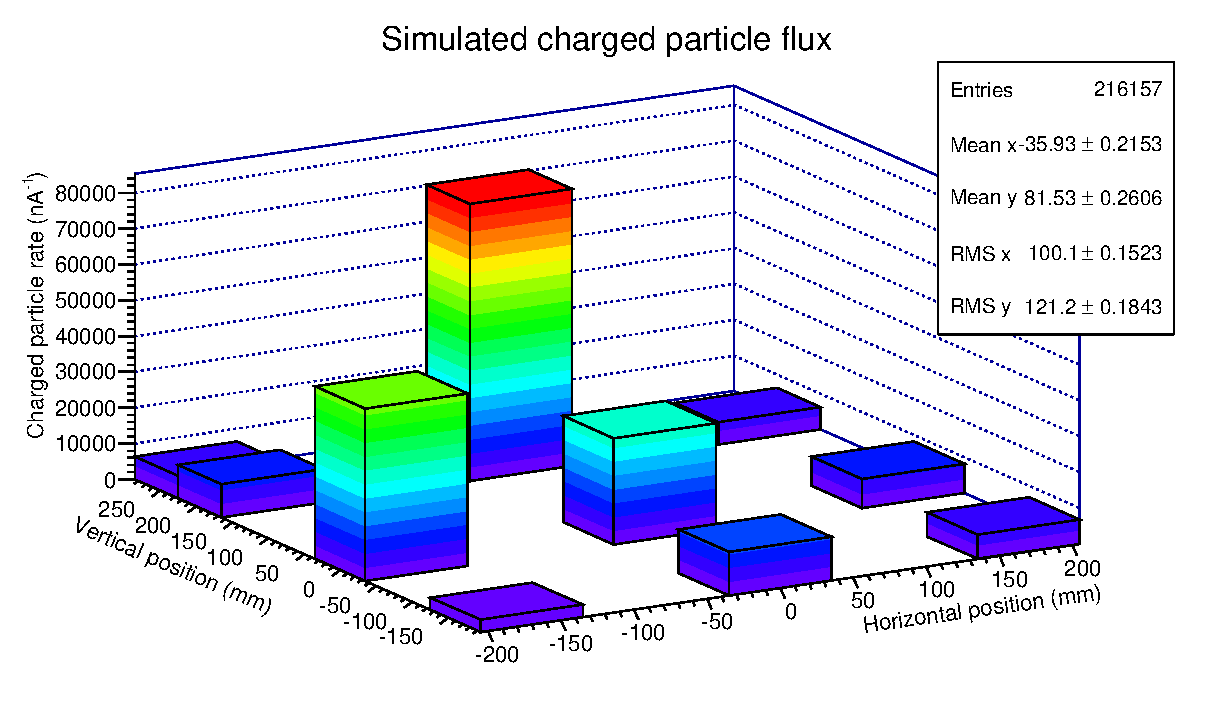
\includegraphics[width=.9\textwidth]{images/plot_generating_scripts/sim_2d_charged_flux.eps}
  \caption{Simulated results for the 2D charged particle rate normalised to a proton current of 1~nA. Colour is equal to the rate as given by the z-axis. Simulated using \( 9\times10^8 \) in G4BL, the rate was taken to be those particles seen within the area of the scintillator used.}
  \label{fig:sim_2d_charged_flux}
\end{figure}

% section analysis (end)
\clearpage
% chapter charged_particle_flux (end)

\section{Muon Lifetime} % (fold)
\label{cha:muon_lifetime}
Measurement of the muon lifetime was done to confirm the presence of muons in the beam. As has been discussed muons have a relatively long lifetime (\(2.197~\mu\)s) that is reasonably distinct from any others; this acts as a useful method of identification. To make the measurement two scintillators are placed on either side of a stopping target. The entire detector is placed perpendicular to the muon's direction of travel. The muons lose energy as they traverse the stopping target and some number of them will decay emitting an electron. By measuring the time differences between a detection at the upstream scintillator (the muon) and a detection at the downstream scintillator (the decay electron) we can spectrum the characteristic exponential decay and measure the muon lifetime. The curve produced is the sum of the many exponentials, each corresponding to the material in which negative muons were captured or the free decay of positive muons. As negative muons are less common at MuSIC than positive ones and because in many materials negative muons have similar lifetimes only two exponentials are typically used: one for the positive muons and another for negative muons captured by the stopping target which has a measurably different lifetime.

In total three measurements of the muon lifetime were taken: one concurrently with the 2D charged particle flux measurement, a high-statistics run and then measurements that form the basis of the muon momentum spectrum measurement. The first two of these measurements will be discussed here and the final one will be discussed later.

\subsection{Experimental Set Up} % (fold)
\label{sec:experimental_set_up}
The basic experimental set up for muon lifetime measurement has already been discussed: two scintillators sandwiching a stopping target. Both measurements were made using the same scintillator and stopping target: two \( 380\times50\times3.5 \)~mm\(^3\) scintillators and a \( 370\times80\times6 \)~mm\(^3\) pure copper target. An MPPC was mounted at either end of both scintillators (4 MPPCs in total) to provide read-out.

The DAQ used was a simple extension of the previous versions. This time, rather than measuring the time differences between the different individual MPPCs the TDC was used to measure the time between a hit on the upstream scintillator and then a hit on the downstream. A `hit' was considered to be a co-incident signal on both MPPCs of that scintillator. As a measure to reduce spurious signals due to other charged particles, e.g.\ electrons, a veto window of 50~ns was used. The veto window was a period following the upstream hit in which no hits were allowed in the downstream scintillator. The veto-window is used to reject particles that didn't decay between the scintillators or which decay but aren't muons (e.g.\ pions, which have a 26~ns lifetime).

% section experimental_set_up (end)
\subsection{Results} % (fold)
\label{sec:results} 
Figures~\ref{fig:music2_mu_lifetime} and \ref{fig:music3_muon_lifetime} show the TDC measurements that were made to record the muon lifetime. The TDC bin values are converted to ns using:
\begin{align}
  t = K(T - T_0)
\end{align}
where \(t\) is the real time, in ns, \(K\) is the calibration constant (0.025, measured by manufacturer), \(T\) is the value recorded in the MH-TDC and \(T_0\) is the time when the start signal for the TDC was sent, as recorded by the MH-TDC on a dedicated channel.

The data is then fitted with either one or two exponential decay functions and a flat background. Whether a single or double exponential is used depends heavily on the amount of data that was taken. A single function was used to fit the free decay of muons (neglecting the captured negative muons) whereas a second exponential was used to model the decay of captured negative muons inside the stopping target. Fitting the copper-decay exponential requires much more data as a significant proportion of the events from this are ignored because of the veto-window. In the first 50~ns \(\sim\)26~\% of all copper decays will have already occurred in comparison to only \(\sim\)2\% of free muon decays, this is made worse as the number of positive muons is significantly higher than the number of negative muons making the captured muon signal much lower.

\begin{figure}[hptb]
  \centering
  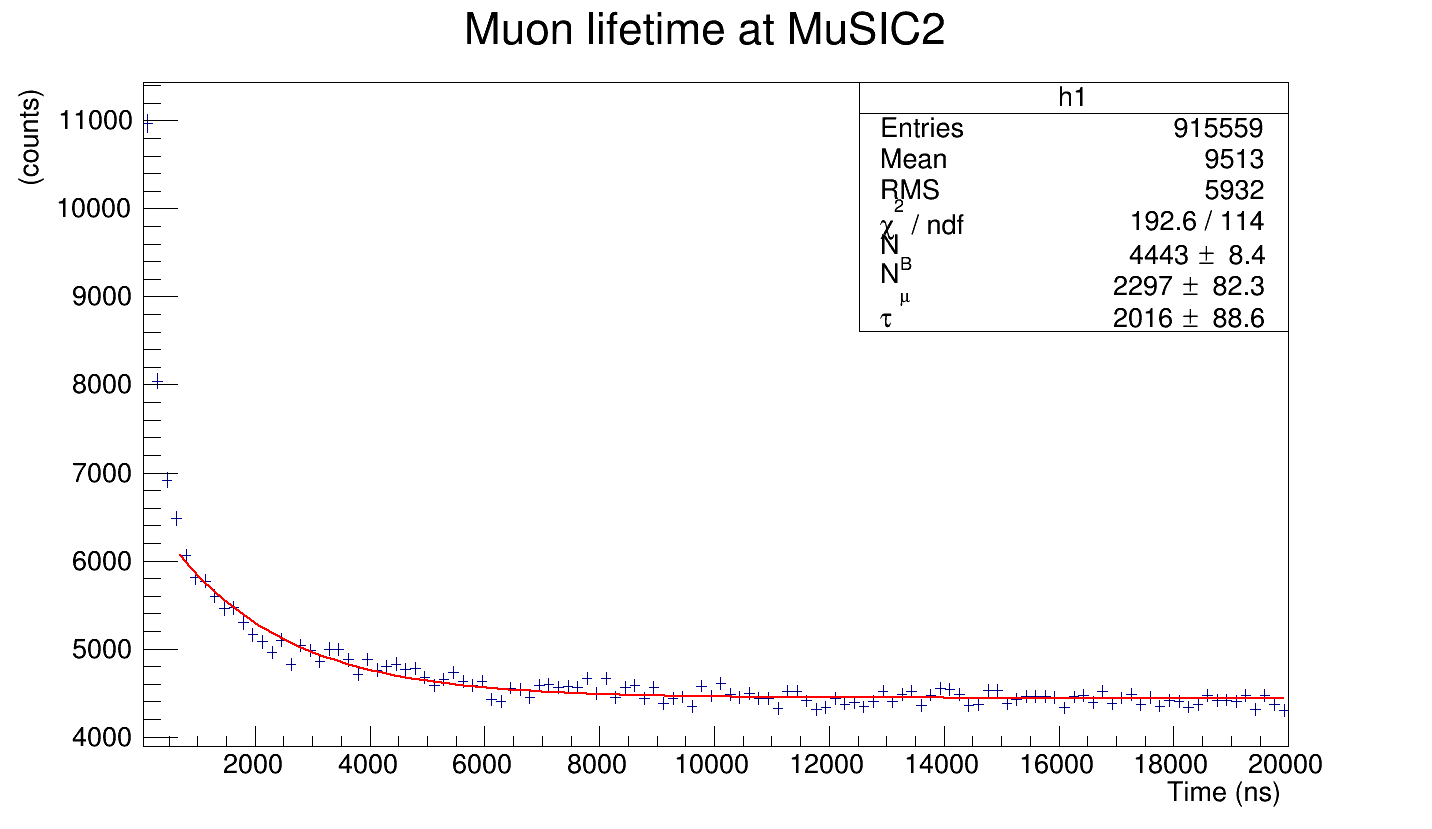
\includegraphics[width=.9\textwidth]{images/lifetime/music2_mu_lifetime_good.png}
  \caption{Results of the first measurement of the muon lifetime. The data was binned in 166~ns bins to remove the affects of noise on the data, only entries with an ADC value of 1,100 (which excluded the pedestal) were used. The fit was applied from 600~ns to 20~\(\mu\)s.}
  \label{fig:music2_mu_lifetime}
\end{figure}

% section results (end)
\subsection{Analysis} % (fold)
\label{sec:analysis}
As can be seen in figures~\ref{fig:music2_mu_lifetime} and \ref{fig:music3_muon_lifetime} the exponential decays are good fits to the data with reasonable chi-squared values (\(192.6/114\) and \( 516/231 \) respectively). The muon lifetimes measured are in reasonable agreement with the canonical value of \((2.1969811\pm0.0000022)\)~\(\mu\)s~\cite{pdg}. The lifetime measurement for the first run is low but this is to be expected as the fit doesn't account for the capture of negative muons which have a much shorter lifetime. Whilst both measurements have a large amount of background this does not remove from the core fact that large numbers of muons were detected and they exhibited the expected properties. The second measurement also produces a measurement of the muonic-copper lifetime which slightly higher than the \((163.5\pm1)\)~ns~\cite{suzuki_mu_capture_rates} measured by others but this discrepancy is small (\(<2\sigma\)) likely due to the presence of contaminating materials (e.g.\ the scintillator plastic).

\begin{figure}[hptb]
  \centering
  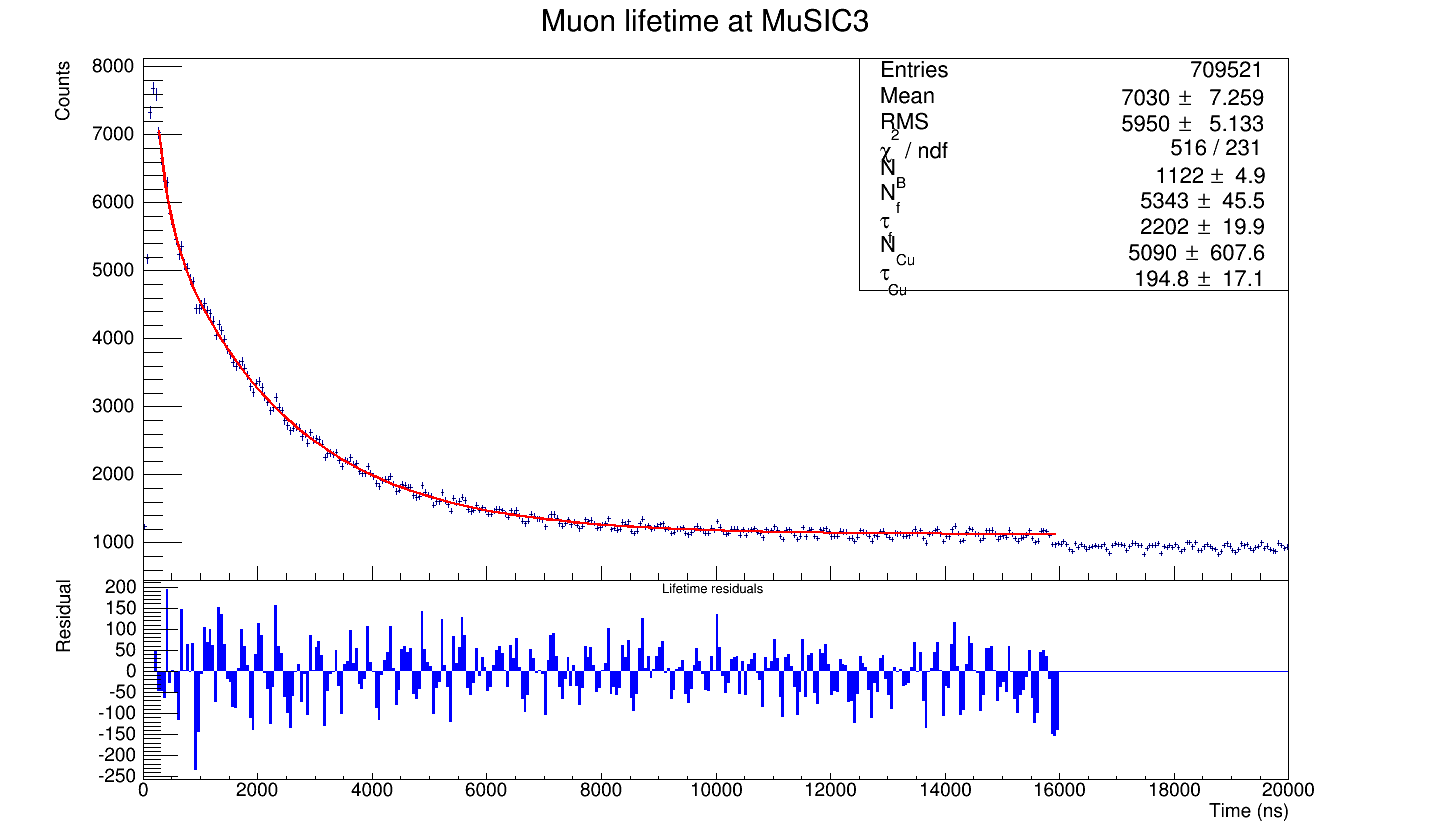
\includegraphics[width=.9\textwidth]{images/lifetime/music3_muon_lifetime.png}
  \caption{Results of the second measurement of the muon lifetime. The data was split between bins with a width of 50~ns and the data was fitted for values between 200~ns and 16~\(\mu\)s. The upper limit of the fit was lowered from the maximal 20~\(\mu\)s due to a fault that caused events to be missed at about 16~\(\mu\)s, as can be seen in the discontinuity at that point.}
  \label{fig:music3_muon_lifetime}
\end{figure}

% section analysis (end)

\clearpage
% chapter muon_lifetime (end)
\section{Momentum Spectrum} % (fold)
\label{cha:momentum_spectrum}
Measurement of the muon momentum spectrum was carried out using an extension of the muon lifetime measurement technique. The number of scintillators was increased to improve coverage of the beam-pipe. To make the momentum measurement, a range of degraders were used to select different (initial) ranges of muon momenta that would then stop. To determine the relation between degrader and stopped muon momentum the simulation was used.

% The final experiment carried out at MuSIC that we will discuss is the measurement of the muon momentum spectrum. The experiment was also extended so that rather than a single narrow scintillator several scintillators forming a basic hodoscope were employed giving coarse vertical flux information as well the desired momentum measurements.

\subsection{Experimental Set Up} % (fold)
\label{sec:experimental_set_up}
\subsubsection{Detector} % (fold)
\label{sub:detector}
The detector consisted of an aluminium degrader whose thickness could be varied to select different momentum ranges, a thin (0.5~mm) upstream counter and a thicker (3.5~mm) downstream counter on either side of a 0.5~mm copper stopping target, table~\ref{tab:detector_dimensions} gives details of the dimensions used. A schematic of the detector can be seen in figure~\ref{fig:m5_setup}. Based on simulation (see chapter~\ref{prt:simulation}) we predicted the mean initial momentum of muons that decay for different degrader thicknesses, the initial muon momentum distribution is given in figure~\ref{fig:images_momentum_spectrum_muon_momentum_at_beam_pipe_exit} and the momentum distributions for the muons that stop in the detector can be seen in figure~\ref{fig:images_momentum_spectrum_stopped_muon_momentum}, the mean momentums are also tabulated in table~\ref{tab:stopped_muon_mom}.
\begin{table}
  \begin{center}
  \begin{tabular}{l | c | c | c | c | c}
    \multirow{2}{*}{Component}  &  \multirow{2}{*}{Material}  
                                            &  \multicolumn{3}{c|}{Dimensions (mm)}  &  \multirow{2}{*}{Number} \\
                                &           &      X      &      Y     &       Z     &                          \\
    \hline
    Degrader                    &    Al     &     400     &     400    &  0.5, 1, 5  &  1                       \\
    Upstream scintillator       &  EJ-212   &     380     &     30     &      0.5    &  8                       \\    
    Stopping Target             &    Cu     &     370     &     310    &      0.5    &  1                       \\    
    Downstream scintillator     &  EJ-212   &     380     &     50     &      3.5    &  5                       \\    
  \end{tabular}
  \end{center}
  \caption{Dimensions of the various detector components. The `Z' is the beam direction, `Y' is vertical and `X' is horizontal. The layout of the detector can be seen in figure~\ref{fig:m5_setup}.}
  \label{tab:detector_dimensions}
\end{table}

\begin{figure}[htbp]
    \centering
        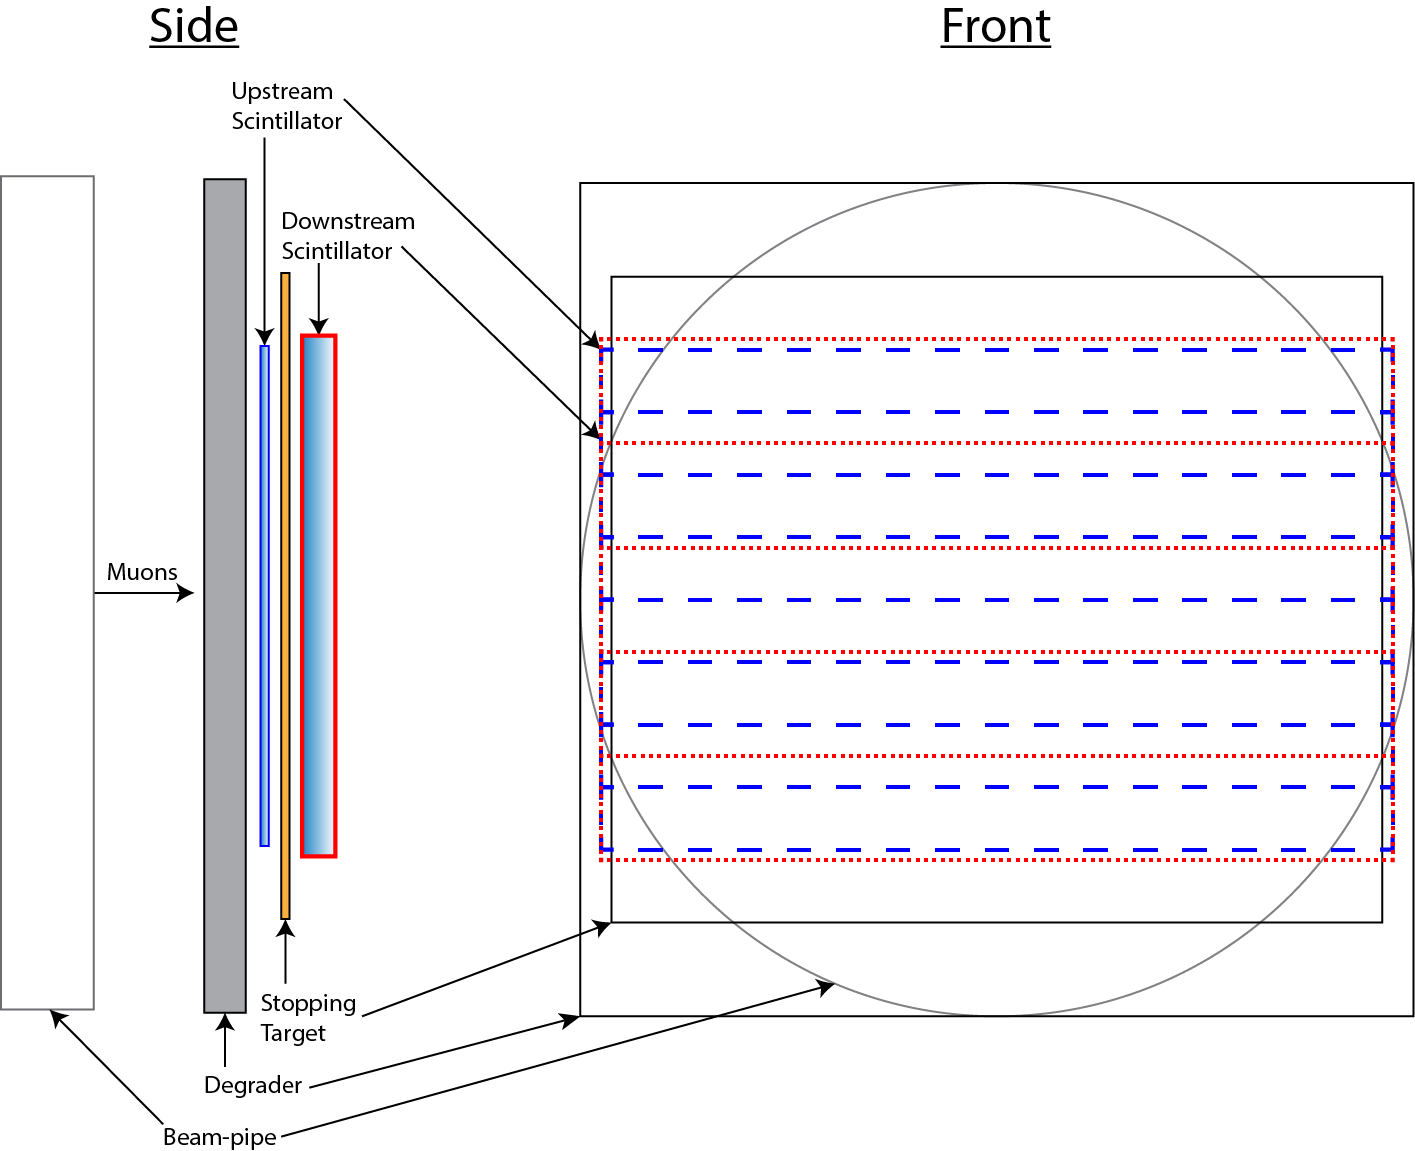
\includegraphics[scale=0.5]{images/momentum_spectrum/Detector_setup_music5.png}
    \caption{Experimental set up of the detector for MuSIC~5 (widths not to scale), see table~\ref{tab:detector_dimensions} for actual sizes. The upstream scintillators are outlined with blue dashes whilst the downstream ones are red dots.}
    \label{fig:m5_setup}
\end{figure}  

\begin{figure}[hptb]
  \centering
    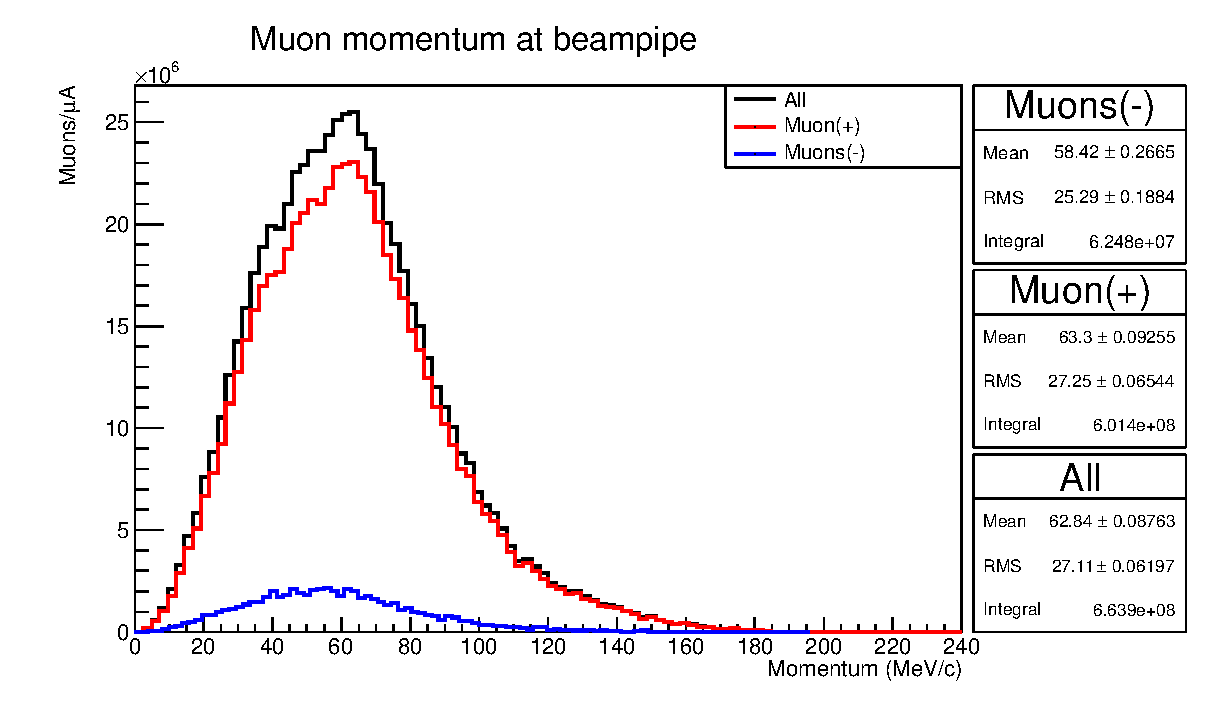
\includegraphics[width=.9\textwidth]{images/momentum_spectrum/muon_momentum_at_beam_pipe_exit.eps}
  \caption{Total muon momenta at the end of the beam pipe. The number of initial muons simulated was 95,700. The plot has been normalised to the number of muons per \(\mu\)A of proton beam.}
  \label{fig:images_momentum_spectrum_muon_momentum_at_beam_pipe_exit}
\end{figure}

\begin{figure}[hptb]
  \centering
    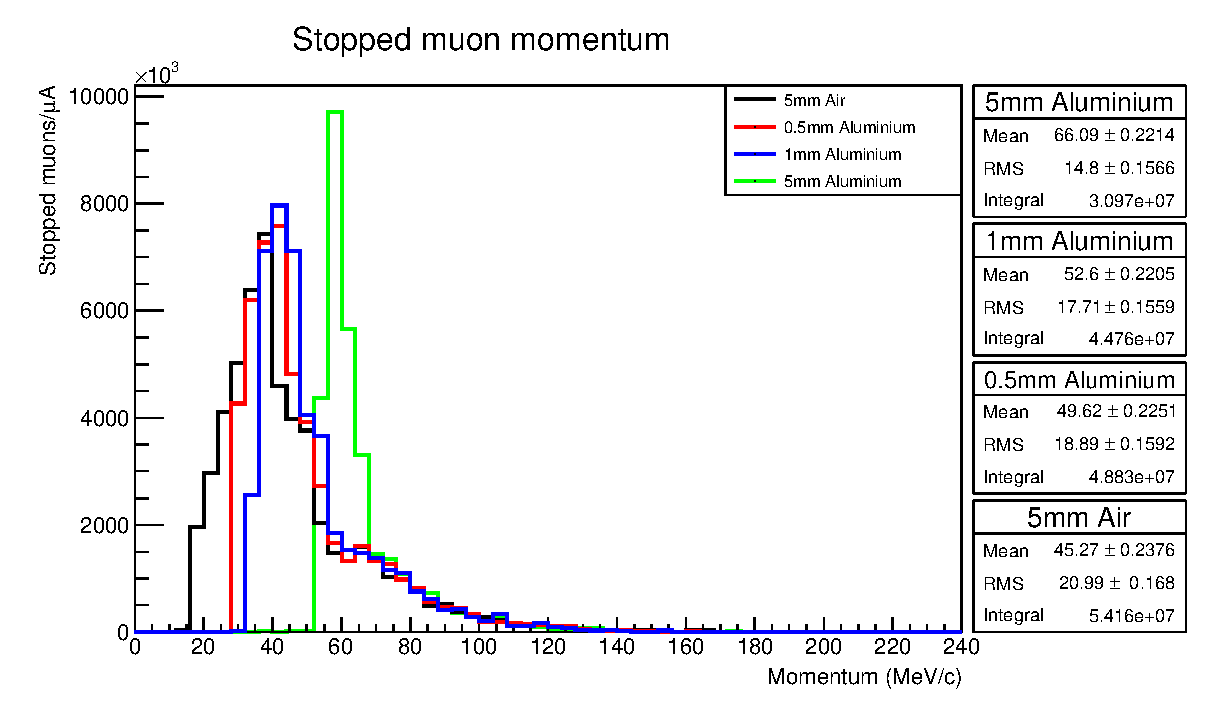
\includegraphics[width=.8\textwidth]{images/momentum_spectrum/stopped_muon_momentum.eps}
  \caption{Momenta at the end of the beam pipe of muons that subsequently stopped. This shows the momenta that the different degraders `select'. The number of initial muons simulated was 95,700. The plot has been normalised to the number of muons per \(\mu\)A of proton beam.}
  \label{fig:images_momentum_spectrum_stopped_muon_momentum}
\end{figure}

\begin{table}
  \lineup
  \begin{center}
  \begin{tabular}{c | r@{\(\pm\)}l | r@{\(\pm\)}l }
    Degrader  &  \multicolumn{4}{c}{Momentum (MeV/c)}      \\
      (mm)    &  \multicolumn{2}{c|}{Mean}  
                               &  \multicolumn{2}{c}{RMS}  \\
    \hline
      0.0     &  45.27 & 0.24  &  20.99 & 0.17             \\
      0.5     &  49.62 & 0.23  &  18.89 & 0.16             \\
      1.0     &  52.60 & 0.22  &  17.71 & 0.16             \\
      5.0     &  66.09 & 0.22  &  14.80 & 0.16             \\
  \end{tabular}
  \end{center}
  \caption{Simulated mean and Root Mean Squared (RMS) momenta of muons, that subsequently stop, at the end of the beam pipe. The degrader is the thickness of the aluminium, the width and height are both 400~mm. The Geant4 simulation was used; in total 95,700 initial muons were simulated, for further details see chapter~\ref{prt:simulation}.}
  \label{tab:stopped_muon_mom}
\end{table}

The counters used were mylar wrapped scintillators with read-out performed by MPPCs mounted on either end of a wavelength shifting fibre bounded along the long axis of the scintillator using optical cement. The signals from each pair of MPPCs are combined and amplified before being passed to the data acquisition system (DAQ) for processing.

Two important considerations were made with the choice of scintillators: the upstream scintillator had to minimise perturbation of the beam whilst providing a suitable trigger from muons and the downstream scintillator had to be effective at detecting electrons. To this end a thin (0.5~mm) upstream scintillator and thicker (3.5~mm) downstream scintillator were chosen. One downside of this set up is that in using a thin upstream scintillator the efficiency for detecting minimally ionising particles is reduced but as only stopping muons were desired this has a negligible effect.

\subsubsection{Data Acquisition} % (fold)
\label{sub:data_acquisition}
The DAQ system used was a simple evolution of that used in the previous experiments: a discriminator unit with paired logic block formed a trigger on a suitably strong upstream signal with no downstream signal within a 50~ns veto window. The triggering signal was recorded using QDC (although it is not analysed here) and a MH-TDC was used to record hit times at all scintillators \(\pm\)20~\(\mu\)s of the trigger. To increase the accuracy of the MH-TDC the trigger time is recorded on a separate channel to the individual MPPC signals called `TDC0' which can then be removed later.

For a signal to be recorded or used as a trigger the discriminator was set to exclude events with fewer than eight photons in the upstream scintillator and fewer than ten in the downstream. The reason for these high values is that each analogue signal, as passed to the discriminator, is the combination of the signals from both the MPPCs on a scintillator. The thinner upstream scintillator has a lower threshold as it's aimed at selecting slow muons that will stop, unfortunately this means it cannot detect mips but these are unlikely to stop. Conversely the downstream scintillator has been set up to select electrons which will deposit more energy and the higher threshold will help reduce background.

A scaler was used to record system diagnostics through regular polling. The values recorded were:
\begin{enumerate}
  \item SEC output.
  \item Triggers (i.e.\ \textsc{u and }\(\overline{\textsc{d}}\)\textsc{ and }\(\overline{\textsc{busy}}\)\footnote{Where `\textsc{u}' is a suitable upstream signal, `\textsc{d}' is a signal in the downstream scintillator and `\textsc{busy}' indicates that the system is busy. Barred values indicate negation, i.e.\ \(\overline{\textsc{d}}\) indicates no downstream signal and \(\overline{\textsc{busy}}\) indicates that the system isn't busy.}).
  \item Potential triggers (i.e.\ \textsc{u and }\(\overline{\textsc{d}}\)).
  \item A clock (for accurate run measurement).
\end{enumerate}
Obviously the clock and SEC were used for normalisation whilst the triggers and potential triggers were used for calculation of dead time (see section~\ref{sub:dead_time}).

% subsection data_acquisition (end)
% section experimental_set_up (end)
\subsection{Data Processing} % (fold)
\label{sec:data_processing}
There were five stages in preparing the data for analysis: reading from VME, calibration and binning. At the end of these processes the data was analysed and the final measurements made. Six data sets were chosen for this analysis, the run conditions are listed in table~\ref{tab:run_summary}.

\begin{table}
	\begin{center}
	\begin{tabular}{c|c|c|c}
		Run ID & Time (sec) & Current (pA) & Degrader (mm) \\
		\hline
		448    & 9,221      & 15           & 0.0   \\
		451    & 1,001      & 15           & 0.5   \\
		452    & 4,924      & 13           & 0.5   \\
		455    & 6,307      & 13           & 1.0   \\
		458    & 5,144      & 14           & 5.0   \\
		459    & 2,452      & 12           & 5.0   \\
	\end{tabular}
	\end{center}
	\caption{Summary of the runs selected for this analysis. The degrader used aluminium and the stopping target 0.5~mm copper.}
	\label{tab:run_summary}
\end{table} 

The data was read from VME using the MIDAS program (`a general purpose data acquisition system for small and medium scale experiments'~\cite{midas_daq}), this dealt with the low level interface to CAMAC and allowed basic plotting of the information.

Once the data was saved, it was calibrated to convert it to convert it to real world measurements. The calibration formula for the MH-TDC was:
\begin{align}\label{equ:tdc_calibration}
    t'   &= 0.024414(t - \text{TDC0})
\end{align}
where \(t'\) is the calibrated time, \(t\) is the MH-TDC value and TDC0 is the time at which the trigger occurred. The calibration co-efficient of \(0.024414\) was determined using a known clock as input to the MH-TDC and then detecting a set number of ticks that could then be read off as MH-TDC values.

The final stage of data preparation was to bin the data, this was done to make later analysis quicker. Each channel had its MH-TDC times combined in 1~ns bins. This left suitable accuracy whilst vastly reducing the data set's size.

\subsection{Secondary calculations} % (fold)
\label{sec:secondary_calculations}
Using the scaler information two checks could be made: the dead time and the Periodic Trigger Rate (PTR). The dead time of the system is a measure of how many events are lost because the system is busy. The PTR is a check that the rate of triggering events is reasonably constant, deviations from a constant rate would indicate possible problems with the data.

\subsubsection{Dead time} % (fold)
\label{sub:dead_time}
As was stated in section~\ref{sub:data_acquisition} the scaler was used to record diagnostics on the DAQ. To calculate the dead time, the trigger count and the potential trigger count are needed which can be used thus:
\begin{align}
    \text{Live time} &= \frac{\text{Good Triggers}}{\text{Potential Triggers}} \\
    \text{Dead time} &= 1 - \text{Live Time} \\
\end{align}
Where potential triggers are those with a signal in the upstream scintillator and no corresponding signal downstream within the 50~ns veto window. A good trigger is a potential trigger that occurs without the system being busy. The results of this calculation are given in table~\ref{tab:dead_time}.
\begin{table}
    \begin{center}
    \begin{tabular}{c | c | c | r@{ $\pm$ }l | r@{ $\pm$ }l | r@{ $\pm$ }l | r@{ $\pm$ }l }
        \multirow{2}{*}{Run} 
             &  Degrader  &  Length 
                              & \multicolumn{4}{c|}{Triggers (\(\times10^3\))}
                              & \multicolumn{2}{c|}{Live time}
                              & \multicolumn{2}{c}{Dead time}  \\
             & (mm)       & (s)               
                              & \multicolumn{2}{c|}{Good}
                              & \multicolumn{2}{c|}{Potential}
                              & \multicolumn{2}{c|}{(\%)}
                              & \multicolumn{2}{c}{(\%)}  \\
        \hline
        448  &  0.0  &  9221  &  9653.0 & 3.1   &  15678.8 & 4.0  &  61.57 & 0.03  &  38.43 & 0.025 \\
        451  &  0.5  &  1001  &  767.32 & 0.88  &   1070.4 & 1.0  &  71.69 & 0.11  &  28.31 & 0.107 \\
        452  &  0.5  &  4944  &  3459.9 & 1.9   &   4667.8 & 2.2  &  74.12 & 0.05  &  25.88 & 0.053 \\
        455  &  1.0  &  6307  &  4090.2 & 2.0   &   5372.4 & 2.3  &  76.13 & 0.05  &  23.87 & 0.050 \\
        458  &  5.0  &  5144  &  2049.1 & 1.4   &   2455.0 & 1.6  &  83.47 & 0.08  &  16.53 & 0.079 \\
        459  &  5.0  &  2452  &  915.31 & 0.96  &   1077.5 & 1.0  &  84.95 & 0.12  &  15.05 & 0.121 \\
    \end{tabular}
    \end{center}
    \caption{Dead and live times for each run along with the number of potential and good triggers. Run time is included to show the origin of the different counts.}
    \label{tab:dead_time}
\end{table}
% subsection dead_time (end)
\subsubsection{Trigger Rate} % (fold)
\label{sub:gain_stability}
To ensure that there were no problems during data taking the trigger rate was checked. The trigger rate gives a measure of how consistent the detector was as well as highlighting any possible problems in the run. Each run was split into 100 equal sections and the trigger rate determined using the values recorded by the scaler. The results are plotted in figure~\ref{fig:gain_stability} and fitted with a flat function. As can be seen as the degrader's thickness increases the trigger rate goes down. There are also some peaks in the first run (448), it is unclear what caused this. There are a few brief drops in rate in runs 458 and 459, it is suspected these are due to technical problems (e.g.\ loose cables). This effect is a source of systematic errors but these are small compared to those due to the detector efficiency.
%
\begin{sidewaysfigure}
  % \begin{figure}%[htbp]
      \centering
          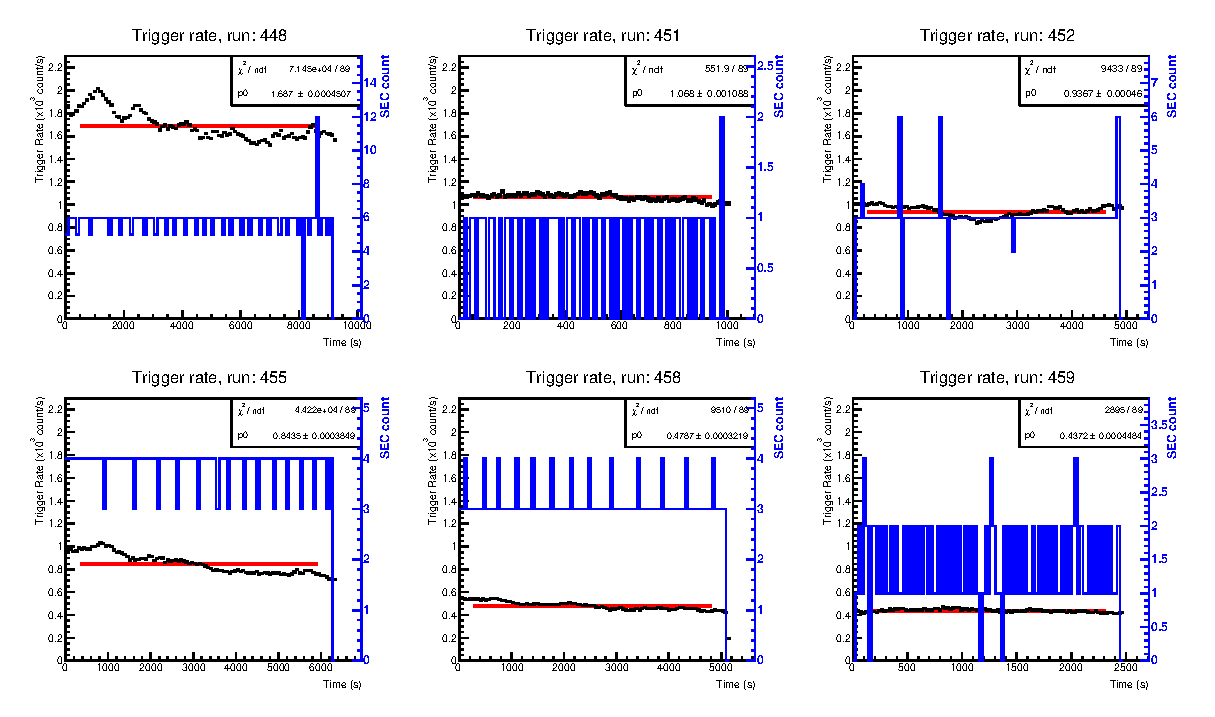
\includegraphics[width=\textwidth]{images/momentum_spectrum/gain_stability.eps}
      \caption{Trigger rate of each run, split over 100 measurements. The triggers used were potential and so exclude any rate limiting due to dead time. The central 90~\% of the data has been fitted with an order 0 polynomial with the parameters given.}
      \label{fig:gain_stability}
  % \end{figure}
\end{sidewaysfigure}

% %
% \begin{table}
%     \begin{center}
%         \begin{threeparttable}
%             \begin{tabular}{c|c|c|c|r@{ $\pm$ }l}
%                 Run & Al degrader thickness (mm) & $\chi^2$ 
%                                                  & N.D.F. \tnote{a}
%                                                  & \multicolumn{2}{|c}{Gain} \\
%                 \hline
%                 448  &  0.0  &  52.94   &  9  &  1.682  &  0.015  \\
%                 451  &  0.5  &  0.8361  &  9  &  1.065  &  0.029  \\
%                 452  &  0.5  &  14.7    &  9  &  0.940  &  0.011  \\
%                 455  &  1.0  &  83.68   &  9  &  0.8331 &  0.0089 \\
%                 458  &  5.0  &  83.41   &  9  &  0.4634 &  0.0055 \\
%                 459  &  5.0  &  1.964   &  9  &  0.4363 &  0.0075 \\
%             \end{tabular}
%             \caption{Gains as determined by the fits to the gain stability in figure~\ref{fig:gain_stability}.}
%             \begin{tablenotes}
%                 \item [a] Number of Degrees of Freedom
%             \end{tablenotes}
%             \label{tab:gain_stability_paramters}
%         \end{threeparttable}
%     \end{center}
% \end{table}

% subsection gain_stability (end)
% section secondary_calculations (end)
\subsection{Results} % (fold)
\label{sec:momenta_results}
As has been discussed there are six data sets that were used for this analysis, the details of them are given in table~\ref{tab:run_summary}. For this analysis only the downstream scintillators are used to calculate the decay times as this was the scintillator best configured to detect them whilst the upstream scintillator was used to form the trigger. Each run was analysed in the same way, once processing was complete (section~\ref{sec:data_processing}) the binned data was converted into a histogram and fitted using:
\begin{align}
  N_{f}\exp\left(\frac{-t}{\tau_{f}}\right) + N_{c}\exp\left(\frac{-t}{\tau_{c}}\right) + N_{s}\sin\left(2\pi\frac{t-\phi}{T}\right) + N_{b} \label{equ:fit}
\end{align}
\(t\) is the time in ns. The four terms each have their own subscript based on what they describe: free muon decay (\(f\)); decay of negative muons captured by the stopping target (\(c\)); a sinusoidal background (\(s\)) and a flat background (\(b\)). The two muon decay terms are parameterised with a scale factor (\(N\)) and a lifetime (\(\tau\)). The sinusoidal term has a period (\(T\)) and phase, relative to the trigger time, (\(\phi\)). 

Originally only a flat background was used but this was found to be insufficient to describe the data and the sinusoidal component was introduced. The sinusoidal effect is thought to be minor bunching of the protons due to the AVF acceleration system which has a stated frequency of 6--18~MHz~\cite{avf_facility} (or a period of 167--56~ns respectively). The flat background is made by travelling particles that don't form a trigger but are recorded by the MH-TDC.

In order to have good statistics whilst maintaining sensitivity to the relatively fast copper component of the decays a bin width of 16~ns was used. A large bin width (e.g.\ 100~ns) could have been used to smooth the sinusoidal noise but this would result in very few bins in which the copper component was significant. Whilst the ideal solution would be to use binning such that the sinusoidal component was cancelled out this was not feasible due to limitations of the fitting program. In the end a bin width was chosen that resulted in a small \(\chi^2\) whilst remaining sensitive to copper.

Fitting all the parameters could not easily be done freely due to the range of values to which it was being fitted; some features (e.g.\ the periodic noise) had a scale of \(\mathcal{O}\)(60)~ns compared to the free decay \(\mathcal{O}\)(2,000)~ns and the entire fit range \(\mathcal{O}\)(20,000)~ns. To mitigate the problem of scale the known values, \(\tau_{f}\) and \(\tau_{c}\), were fixed at their given values of \(2,196.9811\pm0.0022 \)~ns~\cite{pdg} and \( 163.5\pm1 \)~ns~\cite{suzuki_mu_capture_rates} respectively. The period, \(T\), was constrained to \(60\pm5\)~ns which was determined to be a good value from fitting the noise in isolation (see figure~\ref{fig:images_momentum_spectrum_448_D1_noise_fit}).

\begin{figure}[hptb]
  \centering
    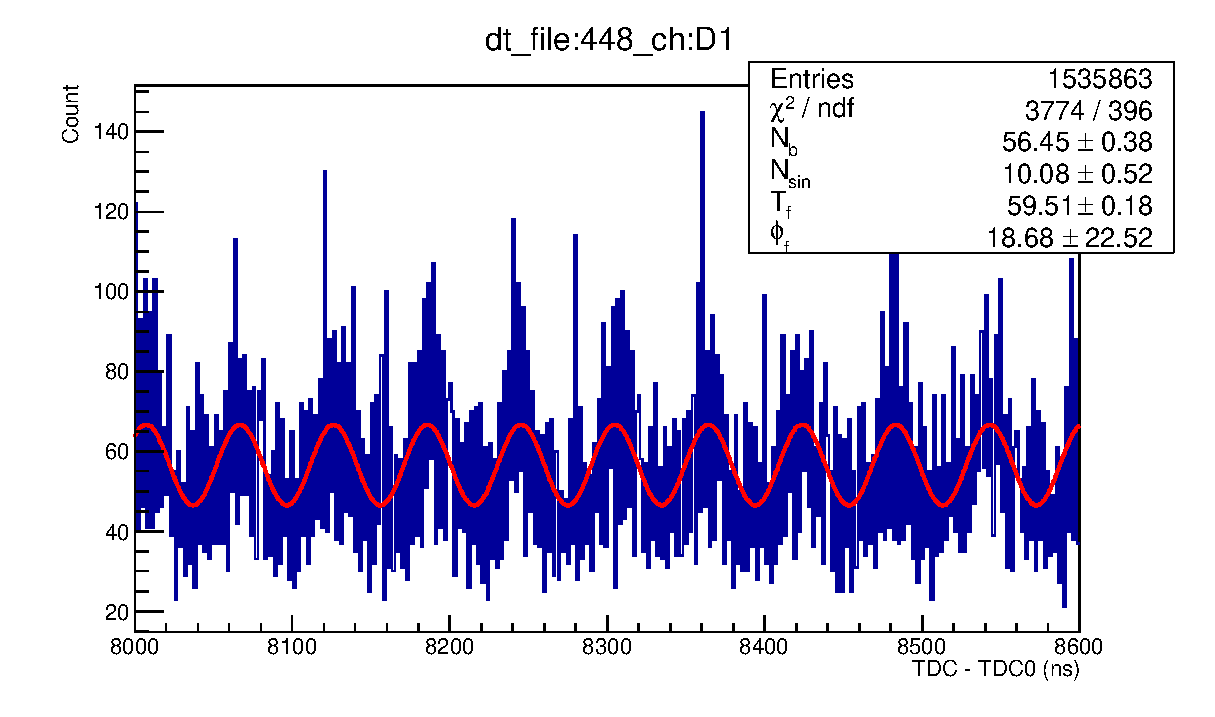
\includegraphics[width=.9\textwidth]{images/momentum_spectrum/448_D1_noise_fit.eps}
  \caption{Zoomed region (8,000~to~8,600~ns) of run 448, channel D1, showing the sinusoidal component of the background, the background has been fitted using \(N_b + N_s\sin(2\pi\frac{t-\phi}{T})\).}
  \label{fig:images_momentum_spectrum_448_D1_noise_fit}
\end{figure}

Once the data was fitted the \(f\) and \(c\) terms were integrated individually to calculate the number of free and copper decays the muons underwent. The fitted histograms are shown in figures~\ref{fig:images_momentum_spectrum_448}~to~\ref{fig:images_momentum_spectrum_459} and the results are summarised in table~\ref{tab:fit_res}. The fitting shows that the bottom channels (D4 and D5) have the worst fit results, often chi-squared values of \(>10,000 / 1,239\)~(ndf), this is compared to values of \(\mathcal{O}(2,000) / 1,239\) for the other channels. Of the other channels D1 and D3 are generally best but D2 is consistently good enough to be useable (unlike channels D4 and D5 which are removed from later analysis).

\begin{table}[hptb]
  \lineup % enable \0, \- & \.
  \begin{center}
  \begin{tabular}{ c | c | r@{\(\,\pm\,\)}l | r@{\(\,\pm\,\)}l | r@{\(\,\pm\,\)}l | r@{\(\,\pm\,\)}l | r@{\(\,\pm\,\)}l }
  % \begin{tabular}{ c | c | S@{\(\pm\)}S | S@{\(\pm\)}S | S@{\(\pm\)}S | S@{\(\pm\)}S | S@{\(\pm\)}S }
    Run  
      &  Ch.  
             & \multicolumn{2}{c|}{\(N_b\)} 
                                 &  \multicolumn{2}{c|}{\(N_s\)}
                                                     &  \multicolumn{2}{c|}{\(\phi\)}  
                                                                         & \multicolumn{2}{c|}{\( N_c \)}
                                                                                           &\multicolumn{2}{c}{\( N_f \)} \\
    \hline
    \multirow{5}{*}{448}
      &  D1  &  576.85\0& 0.80   &  121.10\0& 1.15   &   2.19 & 0.21    &   549\.\0& 31    &  1377.2\0& 5.7  \\
      &  D2  &  914.39\0& 1.0    &  197.28\0& 1.44   &  10.33 & 0.16    &  1524\.\0& 38    &  1937.2\0& 6.9  \\
      &  D3  &  164.22\0& 0.43   &   40.68\0& 0.63   &  18.22 & 0.36    &   592\.\0& 21    &   620.3\0& 3.4  \\
      &  D4  &   32.07\0& 0.19   &    6.89\0& 0.28   &  57.02 & 0.96    &   193\.\0& 11    &   172.8\0& 1.7  \\
      &  D5  &   27.79\0& 0.18   &    6.37\0& 0.26   &   4.31 & 0.94    &    24.8  &\07.8  &    91.1\0& 1.4  \\
    \hline
    \multirow{5}{*}{451}
      &  D1  &   39.55\0& 0.21   &    2.38\0& 0.31   &  25.3\0& 2.4     &    29.4  &\08.1  &   101.4\0& 1.5   \\
      &  D2  &   62.27\0& 0.26   &   17.74\0& 0.38   &  13.28 & 0.50    &   153\.\0& 11    &   178.2\0& 1.9   \\
      &  D3  &   11.52\0& 0.12   &    3.60\0& 0.17   &  20.4\0& 1.2     &    85.6  &\06.5  &    57.76 & 0.99  \\
      &  D4  &    2.18\0& 0.05   &    0.61\0& 0.08   &   6.5\0& 3.0     &    25.9  &\03.5  &    16.59 & 0.49  \\
      &  D5  &    1.97\0& 0.05   &    0.65\0& 0.07   &   8.7\0& 2.6     &     7.3  &\02.6  &     8.78 & 0.40  \\
    \hline
    \multirow{5}{*}{452}
      &  D1  &  161.25\0& 0.43   &   43.56\0& 0.61   &   4.08 & 0.31    &   208\.\0& 17    &   435.5\0& 3.1  \\
      &  D2  &  252.14\0& 0.54   &   71.73\0& 0.76   &  12.39 & 0.25    &   706\.\0& 23    &   789.9\0& 4.0  \\
      &  D3  &   46.29\0& 0.23   &   15.70\0& 0.34   &  19.82 & 0.55    &   335\.\0& 13    &   266.7\0& 2.1  \\
      &  D4  &    8.95\0& 0.11   &    2.49\0& 0.16   &   0.00 & 1.64    &   128.2  &\07.5  &    76.6\0& 1.1  \\
      &  D5  &    8.01\0& 0.097  &    2.37\0& 0.14   &   7.54 & 1.43    &    25.9  &\05.2  &    38.71 & 0.82  \\
    \hline
    \multirow{5}{*}{455}
      &  D1  &  187.67\0& 0.46   &   46.99\0& 0.66   &   4.38 & 0.32    &   265\.\0& 19    &   539.1\0& 3.4  \\
      &  D2  &  293.99\0& 0.58   &   73.76\0& 0.83   &  12.41 & 0.26    &   896\.\0& 26    &   967.9\0& 4.4  \\
      &  D3  &   54.02\0& 0.25   &   17.18\0& 0.37   &  20.27 & 0.53    &   438\.\0& 15    &   326.4\0& 2.3  \\
      &  D4  &   10.37\0& 0.11   &    2.86\0& 0.16   &   0.00 & 0.36    &   195.1  &\08.5  &    87.4\0& 1.1  \\
      &  D5  &    9.30\0& 0.10   &    2.63\0& 0.15   &   4.8\0& 1.3     &    41.9  &\05.8  &    47.00 & 0.90  \\
    \hline
    \multirow{5}{*}{458}
      &  D1  &   73.73\0& 0.29   &   21.53\0& 0.43   &   0.000 & 0.037  &   219\.\0& 15    &   350.2\0& 2.4  \\
      &  D2  &  114.37\0& 0.37   &   34.08\0& 0.54   &   5.32\0& 0.38   &   799\.\0& 20    &   562.4\0& 3.1  \\
      &  D3  &   21.47\0& 0.16   &    8.40\0& 0.24   &   9.89\0& 0.71   &   236\.\0& 11    &   178.1\0& 1.6  \\
      &  D4  &    3.805 & 0.070  &    1.25\0& 0.10   &   0.00\0& 0.19   &    72.6  &\05.8  &    49.23 & 0.80  \\
      &  D5  &    3.728 & 0.067  &    1.436 & 0.098  &   0.00\0& 0.76   &    19.1  &\04.2  &    28.11 & 0.65  \\
    \hline
    \multirow{5}{*}{459}
      &  D1  &   30.67\0& 0.19   &    8.86\0& 0.28   &  56.68 & 0.72    &   115.3  &\09.8  &   155.0\0& 1.6  \\
      &  D2  &   48.07\0& 0.24   &   14.91\0& 0.35   &   4.36 & 0.56    &   369\.\0& 13    &   254.0\0& 2.1  \\
      &  D3  &    8.87\0& 0.11   &    3.65\0& 0.16   &  11.3\0& 1.0     &   110.1  &\07.3  &    81.0\0& 1.1  \\
      &  D4  &    1.631 & 0.046  &    0.579 & 0.068  &  48.2\0& 3.1     &    39.2  &\04.9  &    22.01 & 0.54  \\
      &  D5  &    1.496 & 0.043  &    0.615 & 0.063  &   0.0\0& 1.0     &     8.0  &\02.8  &    12.73 & 0.43  \\
  \end{tabular}
  \end{center}
  \caption{Summary of the fitted values for equation~\eqref{equ:fit}. These are the values used for the calculation of the integrals and, ultimately, the muon rates. The two lifetime parameters, \( \tau_f \) and \( \tau_c \), were fixed at the values \(2,196.9811\pm0.0022 \)~ns~\cite{pdg} and \( 163.5\pm1 \)~ns~\cite{suzuki_mu_capture_rates} respectively, \( T \) was fixed at 60~ns.}
  \label{tab:fit_res}
\end{table}

\begin{sidewaysfigure}
    \centering
      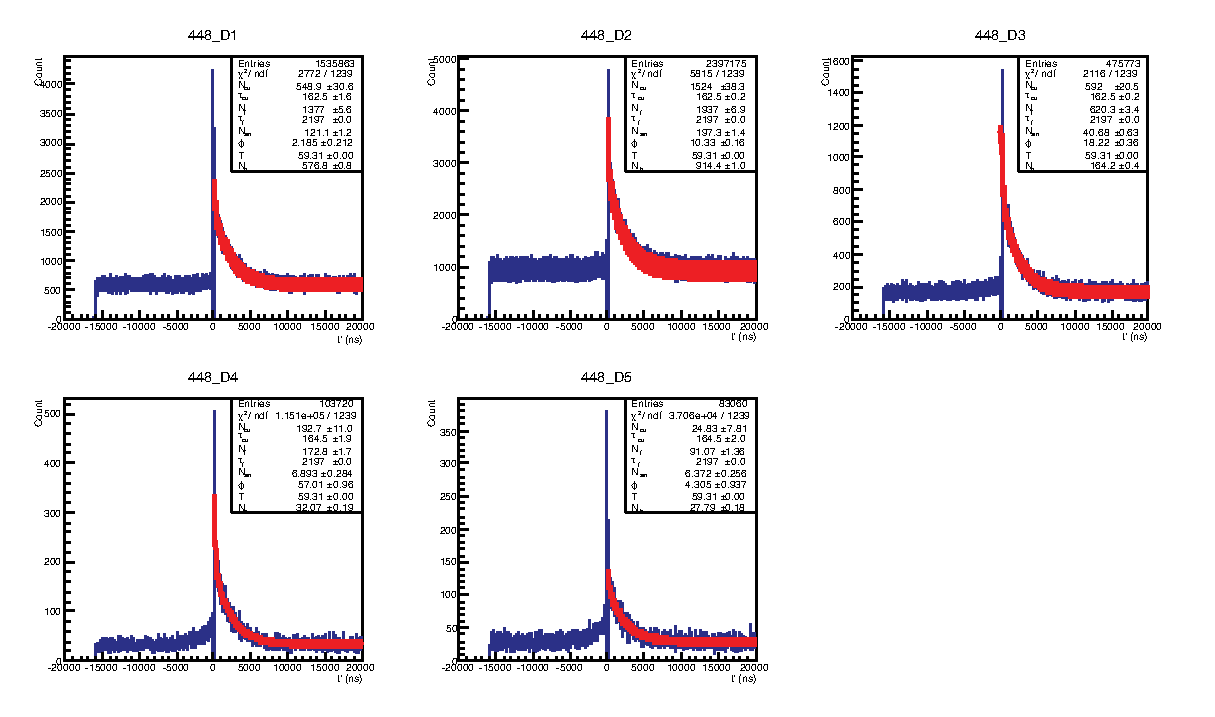
\includegraphics[scale=1]{images/momentum_spectrum/448.eps}
    \caption{Per channel fitting of data for run 448, for this run there was no degrader.}
    \label{fig:images_momentum_spectrum_448}
\end{sidewaysfigure}
%
\begin{sidewaysfigure}
    \centering
      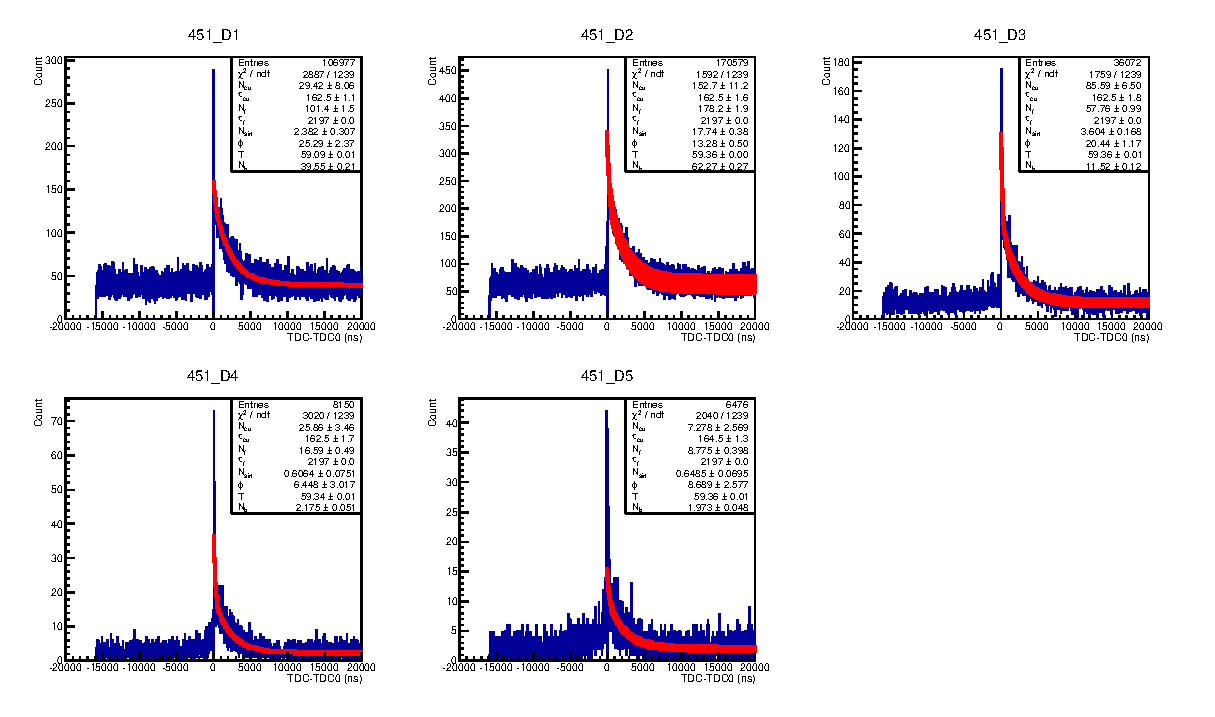
\includegraphics[scale=1]{images/momentum_spectrum/451.eps}
    \caption{Per channel fitting of data for run 451, for this run a 0.5~mm aluminium degrader was used.}
    \label{fig:images_momentum_spectrum_451}
\end{sidewaysfigure}
%
\begin{sidewaysfigure}
    \centering
      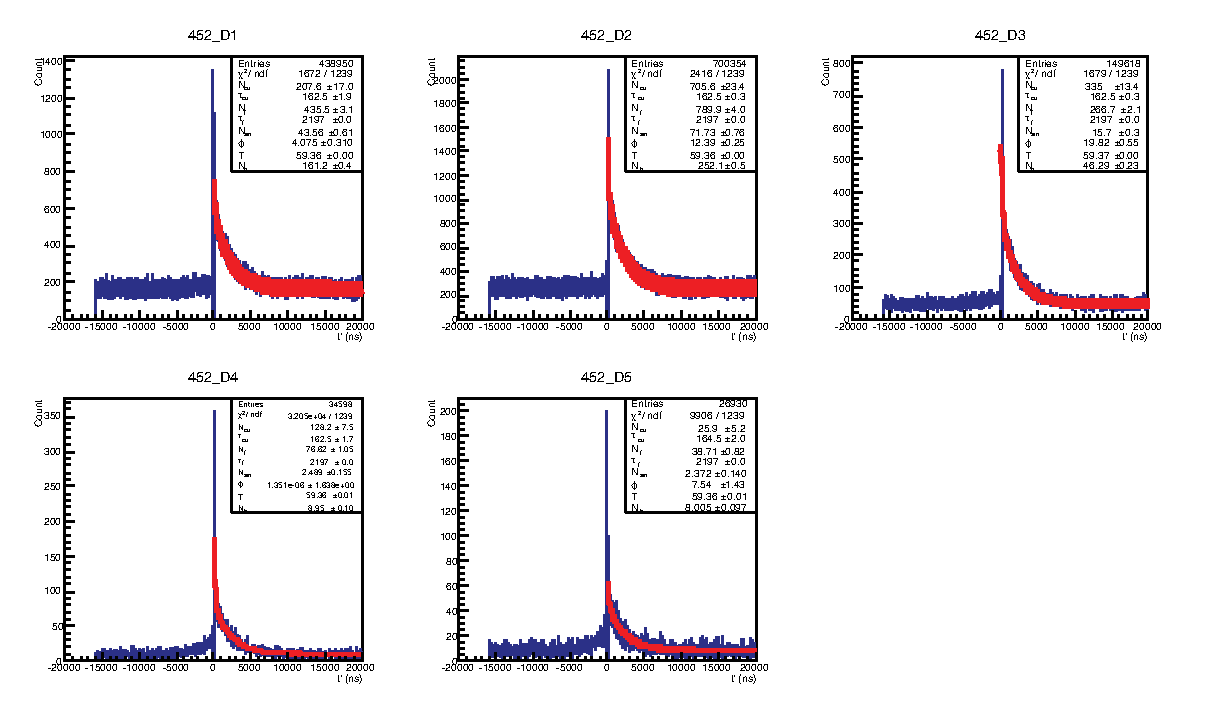
\includegraphics[scale=1]{images/momentum_spectrum/452.eps}
    \caption{Per channel fitting of data for run 452, for this run a 0.5~mm aluminium degrader was used.}
    \label{fig:images_momentum_spectrum_452}
\end{sidewaysfigure}
%
\begin{sidewaysfigure}
    \centering
      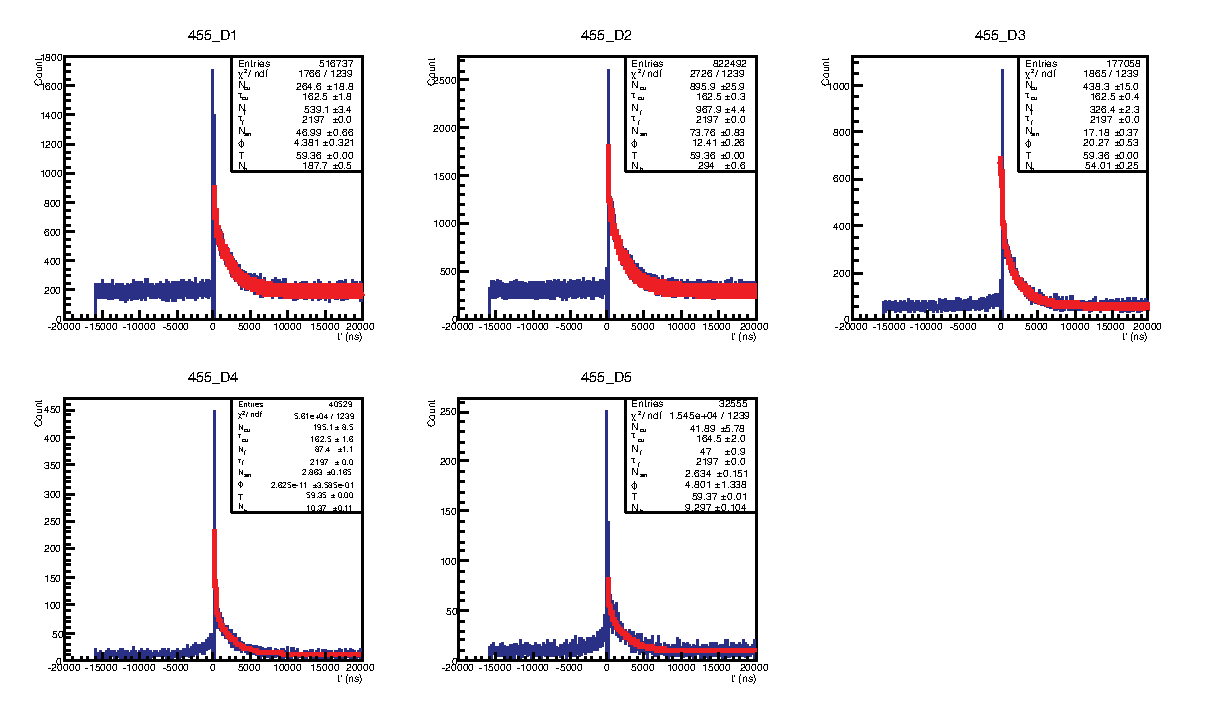
\includegraphics[scale=1]{images/momentum_spectrum/455.eps}
    \caption{Per channel fitting of data for run 455, for this run a 1~mm aluminium degrader was used.}
    \label{fig:images_momentum_spectrum_455}
\end{sidewaysfigure}
%
\begin{sidewaysfigure}
    \centering
      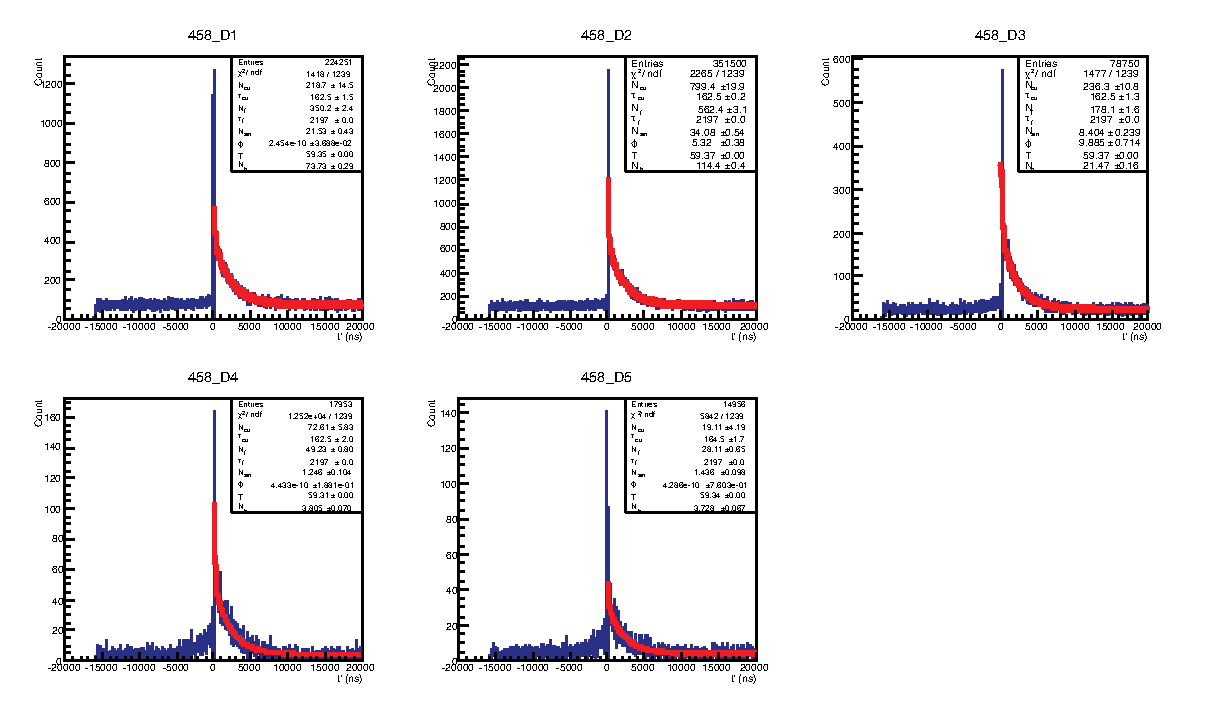
\includegraphics[scale=1]{images/momentum_spectrum/458.eps}
    \caption{Per channel fitting of data for run 458, for this run a 5~mm aluminium degrader was used.}
    \label{fig:images_momentum_spectrum_458}
\end{sidewaysfigure}
%
\begin{sidewaysfigure}
    \centering
      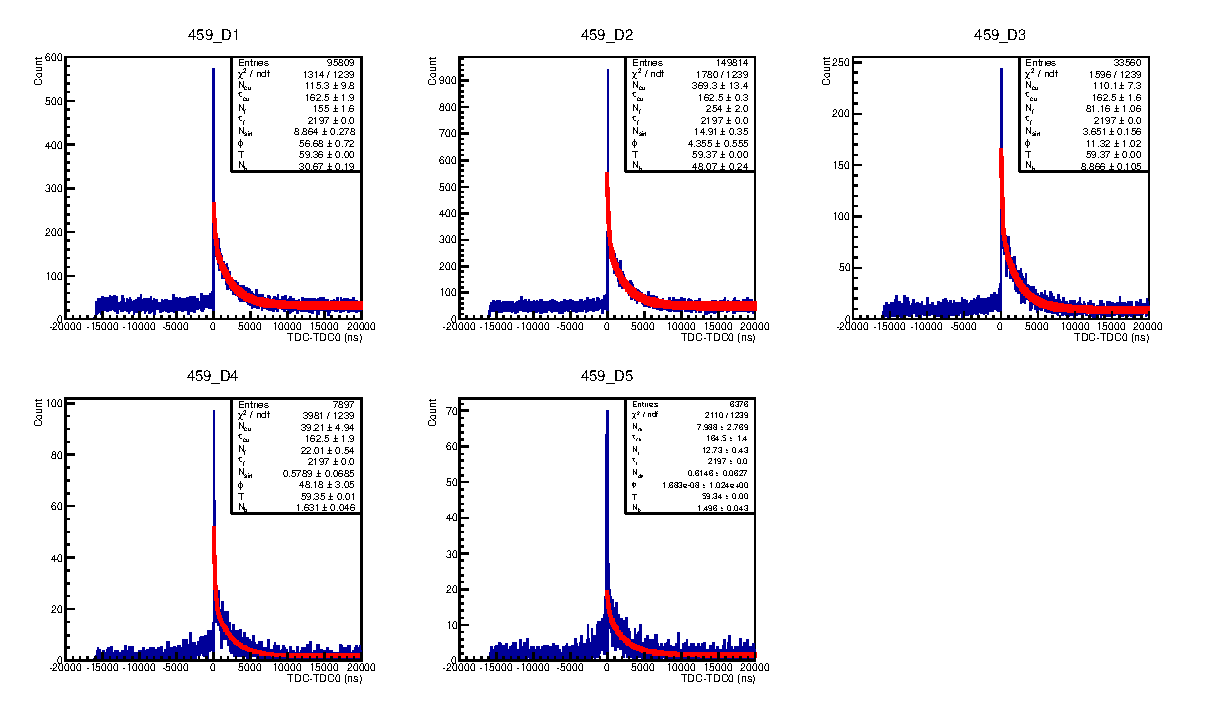
\includegraphics[scale=1]{images/momentum_spectrum/459.eps}
    \caption{Per channel fitting of data for run 459, for this run a 5~mm aluminium degrader was used.}
    \label{fig:images_momentum_spectrum_459}
\end{sidewaysfigure}


\clearpage

Once calculated via integration the number of muons can be summed for all the channels in a run. The summed value can then be normalised between runs to the proton beam current using:
\begin{align}
  R &= \frac{N_{\mu}}{I_p T L} \label{equ:rate}
\end{align}
Where \( R \) is the normalised rate of muon decays (in nA\(^{-1}\)), \(N_{\mu}\) is the number of muon decays (either free or from muonic copper), \( I_p \) is the proton current in nA, \( T \) is the duration of the run in seconds and \(L\) is the live time (as given in table~\ref{tab:dead_time}). The rates and number of muon decays, summed over all channels, are given in table~\ref{tab:rates_res}. The results back up the earlier measurements made on the beam flux (section~\ref{cha:charged_particle_flux}) as the larger values of \(N_f\), \( N_c \) and \(N_b\) are seen in channels D1, D2 and D3, i.e.\ the beam position is in the upper portion of the detector.

\begin{table}
  \begin{center}
  \begin{tabular}{c | c | c | c | r@{\(\pm\)}l | r@{\(\pm\)}l | r@{\(\pm\)}l | r@{\(\pm\)}l  }
    \multirow{2}{*}{Run}  &  \(I_{p}\)  &  \(T\)  &  \multirow{2}{*}{\(L\)}  
         &  \multicolumn{4}{c|}{Copper Decays}   
                                          & \multicolumn{4}{c}{Free Decays}\\
                          &  (nA)       &   (s)   &
         &  \multicolumn{2}{c|}{Count}
                         &  \multicolumn{2}{c|}{ Rate (nA\(^{-1}\))}
                                          &  \multicolumn{2}{c|}{Count}
                                                            &  \multicolumn{2}{c}{Rate (nA\(^{-1}\))} \\
    \hline
    448  &  0.01534  &  9221  &  0.6157  &  19895 & 400  &  228.5 & 4.6   &  528076 & 1283  &  6065 & 15  \\
    451  &  0.01546  &  1001  &  0.7169  &   1999 & 114  &  180.2 & 10.3  &   45269 & 355   &  4080 & 33  \\
    452  &  0.01313  &  4944  &  0.7412  &   9319 & 240  &  193.6 & 5.0   &  200246 & 732   &  4161 & 15  \\
    455  &  0.01332  &  6307  &  0.7613  &  11937 & 265  &  186.6 & 4.1   &  246059 & 803   &  3847 & 13  \\
    458  &  0.01363  &  5144  &  0.8347  &   9365 & 202  &  160.1 & 3.5   &  146384 & 570   &  2502 & 10  \\
    459  &  0.01238  &  2452  &  0.8495  &   4440 & 136  &  172.1 & 5.3   &   65781 & 378   &  2550 & 15  \\
  \end{tabular}
  \end{center}
  \caption{Decay counts and rates, summed over all downstream scintillators.}
  \label{tab:rates_res}
\end{table}

Figures~\ref{fig:images_momentum_spectrum_run_muon_rate_in_f}~and~\ref{fig:images_momentum_spectrum_run_muon_rate_in_cu} show the rates of decays from free muons and muonic copper respectively. These plots are the `pure' rates based solely on the measured values. Between the pairs of runs (e.g.\ runs 451/452 and 458/459) there is reasonable agreement and the general shape suggests that (unsurprisingly) as larger degraders are used there are fewer decays of stopped muons. 

\begin{figure}[hptb]
  \centering
    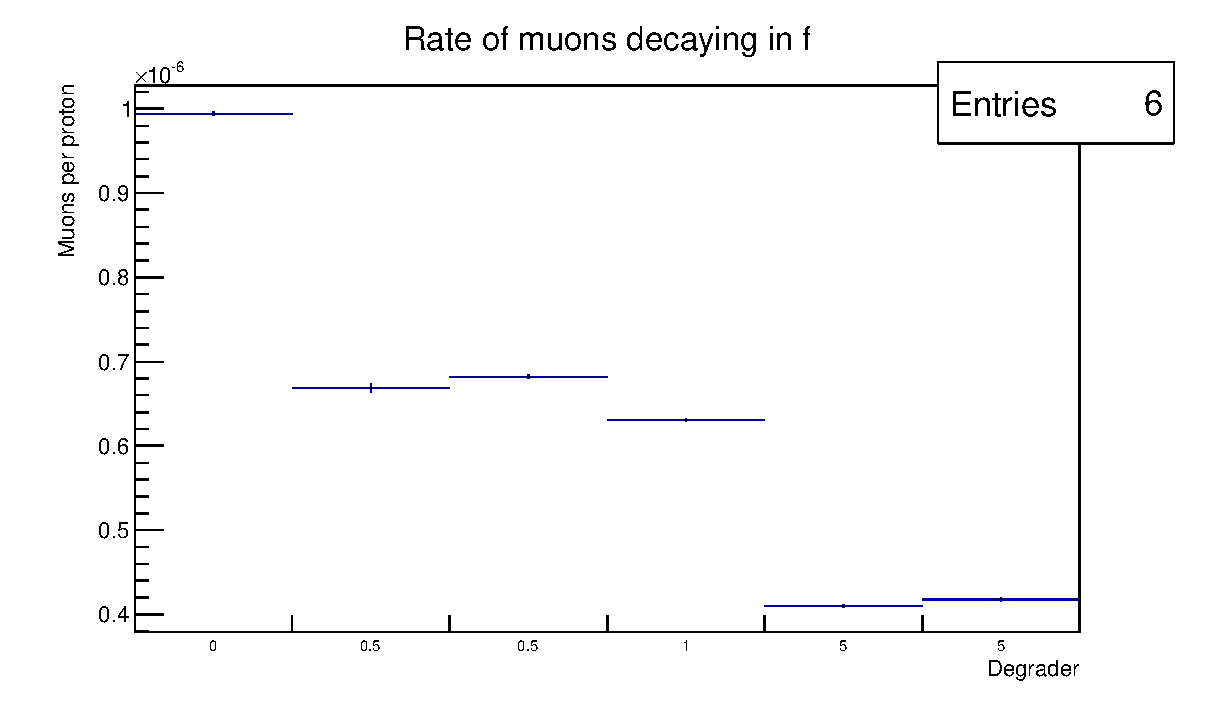
\includegraphics[width=.9\textwidth]{images/momentum_spectrum/run_muon_rate_in_f.eps}
  \caption{Integrated number of free muon decays summed over all channels.}
  \label{fig:images_momentum_spectrum_run_muon_rate_in_f}
\end{figure}

\begin{figure}[hptb]
  \centering
    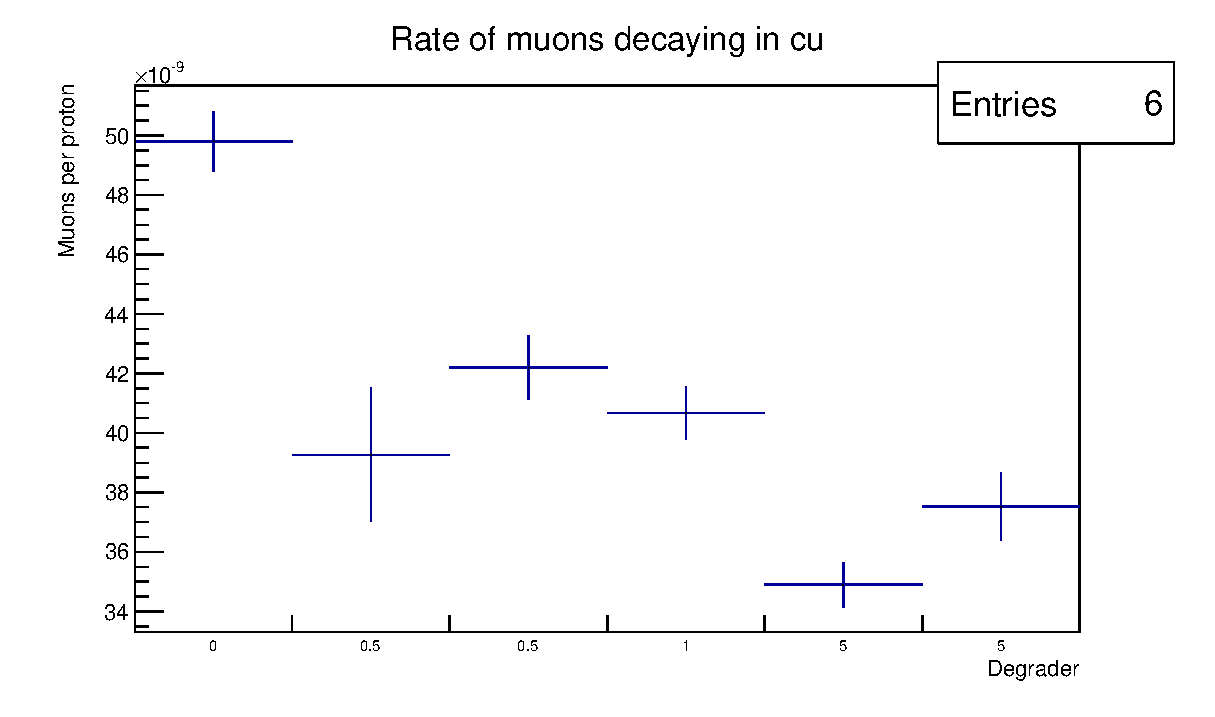
\includegraphics[width=.9\textwidth]{images/momentum_spectrum/run_muon_rate_in_cu.eps}
  \caption{Integrated number of muon decays in copper summed over all channels.}
  \label{fig:images_momentum_spectrum_run_muon_rate_in_cu}
\end{figure}

% As can be seen further refinements can be made to enable more accurate comparison to simulation: inclusion of the acceptance and the detector efficiency as well as conversion of the degrader thickness to the simulated average momentums.

As can be seen in the fit histograms, the \(\chi^2\) values for the fitting of channels D4 and D5 are generally poor and because of this they were removed from the final, summed, rate calculation. The main cause of the poor \(\chi^2\) value is likely the low statistics compounded by the fact that, as the counters share a common trigger those scintillators that are further away from the beam spot will record a greater fraction of noise. Also even for the channels with better \(\chi^2\) values, equation~\eqref{equ:fit} is not a full description of the data. This effect can be seen more clearly when the values for \( \tau_c \) and \( \tau_f \) are also fitted (rather than fixed, as in the analysis). The fitted values for \(\tau_c\) and \(\tau_f\)  are shown in figures~\ref{fig:images_plot_generating_scripts_per_ch_free_lifetime}~and~\ref{fig:images_plot_generating_scripts_per_ch_copper_lifetime} respectively. Both of these plots show that the fitted values differ from the canonical values whilst simultaneously providing a worse \(\chi^2\) than is seen with the constrained values. The poor performance of the fitting when the lifetime values are not fixed is likely a combination of the noisy data and the difficulty of fitting the large number of parameters over a wide range of values (from 1 to 20,000~ns).

\begin{figure}[hptb]
  \centering
    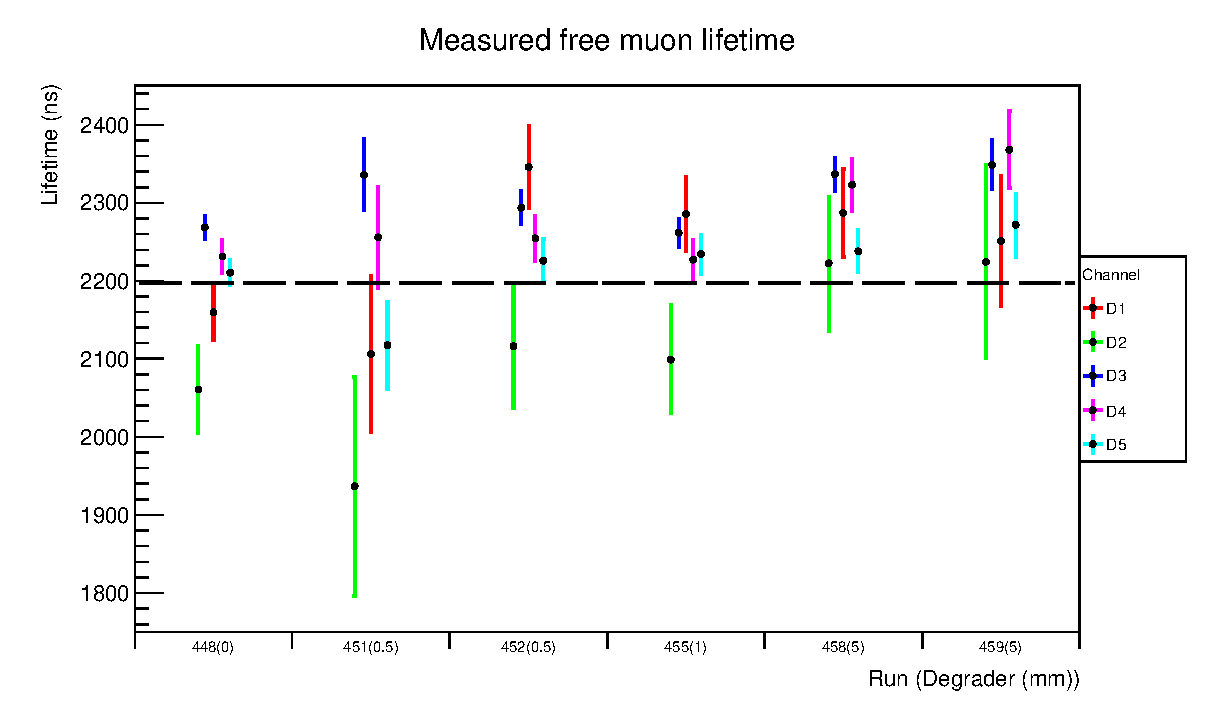
\includegraphics[width=.9\textwidth]{images/plot_generating_scripts/per_ch_free_lifetime.eps}
  \caption{Comparison of fitted value of free muon lifetime for the different channels in each run. The dashed line is the canonical value, \((2.1969811\pm0.0000022)\)~\(\mu\)s~\cite{pdg}.}
  \label{fig:images_plot_generating_scripts_per_ch_free_lifetime}
\end{figure}

\begin{figure}[hptb]
  \centering
    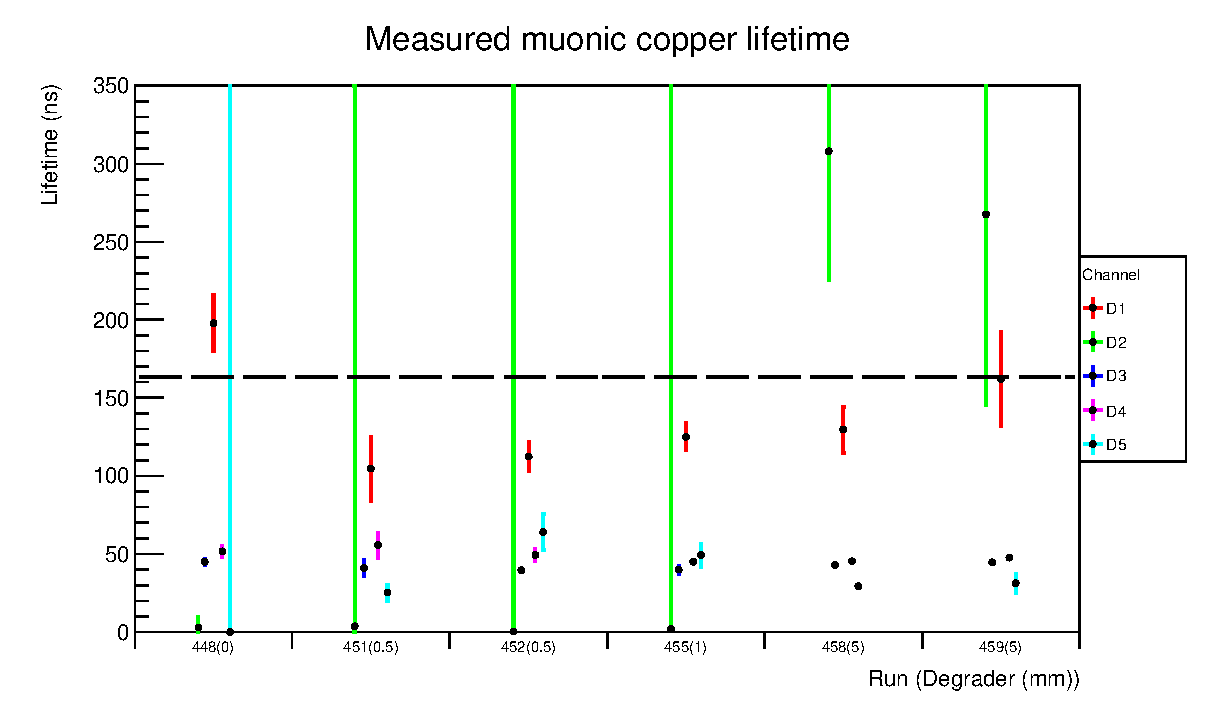
\includegraphics[width=.9\textwidth]{images/plot_generating_scripts/per_ch_copper_lifetime.eps}
  \caption{Comparison of fitted value of muonic copper lifetime for the different channels in each run. The dashed line is the canonical value, \((163.5\pm1)\)~ns~\cite{suzuki_mu_capture_rates}.}
  \label{fig:images_plot_generating_scripts_per_ch_copper_lifetime}
\end{figure}

% \begin{table}
%   \lineup
%   \begin{center}
%   \begin{tabular}{c | c | r@{\(\,\pm\,\)}l | r@{\(\,\pm\,\)}l | r@{\(\,\pm\,\)}l | r@{\(\,\pm\,\)}l | r | l }
%    \multirow{2}{*}{Run} 
%      & \multirow{2}{*}{Channel}
%           &  \multicolumn{2}{c|}{Copper}
%                          &  \multicolumn{2}{c|}{Free}  
%                                           & \multicolumn{2}{c|}{Rate (copper)}
%                                                                  &\multicolumn{2}{c|}{Rate (free)}
%                                                                      &\multicolumn{1}{c|}{\multirow{2}{*}{\(\chi^2\)}}
%                                                                                      & \multicolumn{1}{c}{\multirow{2}{*}{NDF}}  \\ 
%      &    & \multicolumn{2}{c|}{decays}
%                          &  \multicolumn{2}{c|}{decays}  
%                                            & \multicolumn{2}{c|}{(nA\(^{-1}\))}
%                                                                 & \multicolumn{2}{c|}{(nA\(^{-1}\))}
%                                                                                      &         &      \\
%    \hline
%    \multirow{5}{*}{448}
%      & D1 &   4098 & 232  &  184833 & 758  &    47.1\0& 2.7   &  2122.7  &  8.8   &    2772 & 1239  \\
%      & D2 &  11377 & 286  &  259990 & 928  &   130.7\0& 3.3   &  2986\.\0& 11     &    5815 & 1239  \\
%      & D3 &   4420 & 153  &   83253 & 458  &    50.8\0& 1.8   &   956.1  &  5.3   &    2116 & 1239  \\
%      & D4 &   1462 &  85  &   23189 & 228  &    16.79 & 0.98  &   266.3  &  2.6   &  115129 & 1239  \\
%      & D5 &    188 &  59  &   12223 & 183  &     2.16 & 0.68  &   140.4  &  2.1   &   37059 & 1239  \\
%    \hline
%    \multirow{5}{*}{451}
%      & D1 &    220 &  60  &   13602 & 202  &    19.8\0& 5.4   &  1226\.\0& 18    &   2887 & 1239  \\ 
%      & D2 &   1140 &  84  &   23915 & 261  &   102.8\0& 7.6   &  2155\.\0& 24    &   1592 & 1239  \\ 
%      & D3 &    639 &  49  &    7751 & 132  &    57.6\0& 4.4   &   699\.\0& 12    &   1759 & 1239  \\ 
%      & D4 &    193 &  26  &    2227 &  66  &    17.4\0& 2.3   &   200.7  &  6.0  &   3020 & 1239  \\ 
%      & D5 &     55 &  19  &    1178 &  53  &     5.0\0& 1.8   &   106.1  &  4.8  &   2040 & 1239  \\ 
%    \hline
%    \multirow{5}{*}{452}
%      & D1 &   1550 & 128  &   58446 & 413  &    32.2\0& 2.7   &  1214.5  &  8.6  &   1672 & 1239  \\
%      & D2 &   5268 & 175  &  106013 & 538  &   109.5\0& 3.7   &  2203\.\0& 11    &   2416 & 1239  \\
%      & D3 &   2501 & 100  &   35787 & 277  &    52.0\0& 2.1   &   743.6  &  5.8  &   1680 & 1239  \\
%      & D4 &    957 &  57  &   10282 & 141  &    19.9\0& 1.2   &   213.7  &  2.9  &  32046 & 1239  \\
%      & D5 &    196 &  39  &    5195 & 110  &     4.08 & 0.81  &   108.0  &  2.3  &   9906 & 1239  \\
%    \hline
%    \multirow{5}{*}{455}
%      & D1 &   1976 & 142  &   72348 & 453  &    30.9\0& 2.2   &   1131.0 &  7.1  &   1766 & 1239  \\
%      & D2 &   6689 & 194  &  129903 & 589  &   104.6\0& 3.0   &   2030.8 &  9.3  &   2726 & 1239  \\
%      & D3 &   3273 & 112  &   43808 & 304  &    51.1\0& 1.8   &    684.9 &  4.8  &   1865 & 1239  \\
%      & D4 &   1457 &  65  &   11730 & 151  &    22.8\0& 1.0   &    183.4 &  2.4  &  56096 & 1239  \\
%      & D5 &    318 &  44  &    6308 & 121  &     4.97 & 0.69  &     98.6 &  1.9  &  15454 & 1239  \\
%    \hline
%    \multirow{5}{*}{458}
%      & D1 &   1633 & 109  &   46999 & 328  &    27.9\0& 1.9   &    803.4 &  5.7  &   1418 & 1239  \\
%      & D2 &   5968 & 149  &   75477 & 414  &   102.0\0& 2.6   &   1290.2 &  7.2  &   2265 & 1239  \\
%      & D3 &   1765 &  82  &   23907 & 214  &    30.2\0& 1.4   &    408.7 &  3.7  &   1477 & 1239  \\
%      & D4 &    542 &  44  &    6607 & 107  &     9.27 & 0.75  &    112.9 &  1.8  &  12516 & 1239  \\
%      & D5 &    145 &  32  &    3773 &  87  &     2.48 & 0.54  &     64.5 &  1.5  &   5842 & 1239  \\
%    \hline
%    \multirow{5}{*}{459}
%      & D1 &    861 &  74  &   20803 & 216  &    33.4\0& 2.9   &    806.5 &  8.5  &   1314 & 1239  \\
%      & D2 &   2757 & 100  &   34085 & 275  &   106.9\0& 3.9   &   1321.4 & 10.8  &   1780 & 1239  \\
%      & D3 &    822 &  55  &   10893 & 143  &    31.9\0& 2.1   &    422.3 &  5.6  &   1596 & 1239  \\
%      & D4 &    293 &  37  &    2954 &  73  &    11.4\0& 1.4   &    114.5 &  2.8  &   3981 & 1239  \\
%      & D5 &     61 &  21  &    1708 &  58  &     2.35 & 0.81  &     66.2 &  2.2  &   2110 & 1239  \\
%   \end{tabular}
%   \end{center}
%   \caption{Summary of the results of integrating equation~\eqref{equ:fit} and using the values from table~\ref{tab:fit_res}. The rates are the initial values calculated using equation~\eqref{equ:rate}.}
%   \label{tab:rates_res}
% \end{table}

% \begin{figure}[hptb]
%   \centering
%     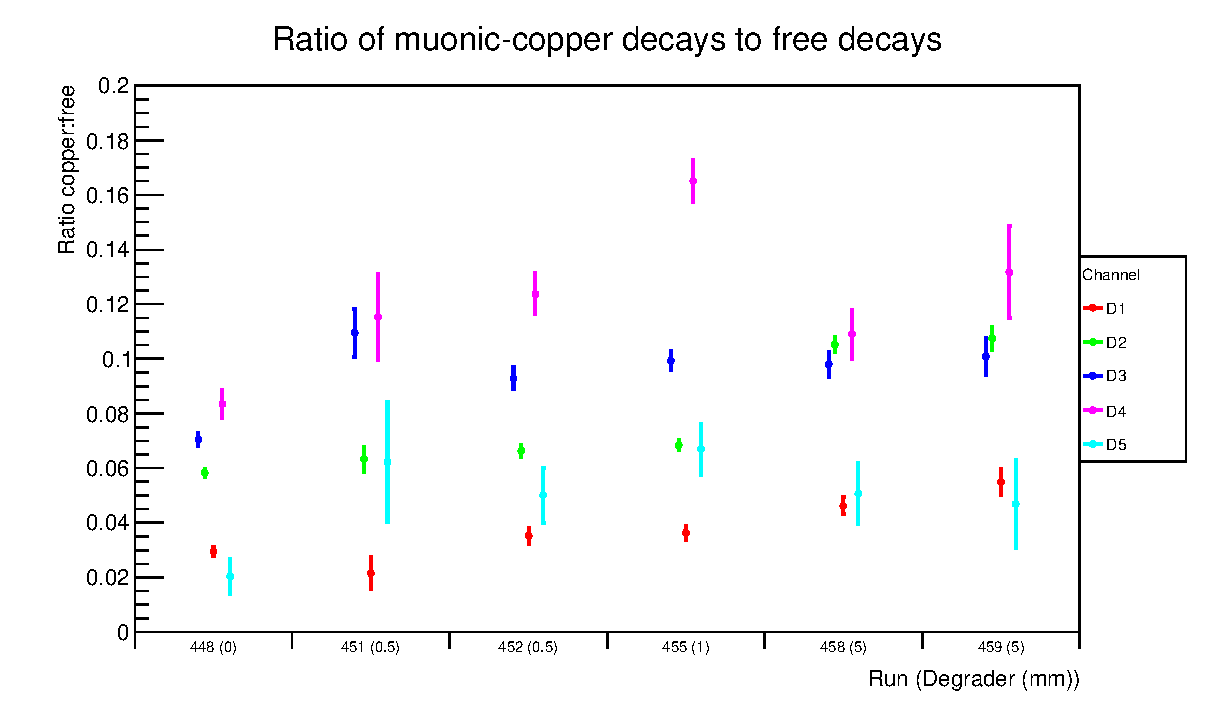
\includegraphics[width=.9\textwidth]{images/plot_generating_scripts/Ratio.eps}
%   \caption{Ratio of copper to free decays. The X-axis shows the degrader thickness whilst the colour indicates channel.}
%   \label{fig:images_plot_generating_scripts_Ratio}
% \end{figure}

\clearpage
Once the muon rates (figure~\ref{fig:images_momentum_spectrum_run_muon_rate_in_f}) have been calculated they can be corrected to account for other effects. This is shown in figure~\ref{fig:images_plot_generating_scripts_adjusted_muon_rates} where additional terms have been incorporated to account for the photon acceptance, the MPPC efficiency and the systematic errors due to the fitting procedure. 

The photon acceptance was calculated using the optical simulation and a simple muon gun particle source. The photon acceptance was defined to be the ratio of muons that decay in a detectable manner (`potential decays') to those that produce photons that are detected (`detected decays'):
\begin{align}
  A &= \frac{\text{Detected decays}}{\text{Potential decays}} \label{equ:photon_acceptance}
\end{align}
A detectable muon was considered to be one that traverses the upstream detector and has a corresponding daughter electron traverse the downstream detector. The requirement for detected photons are that the number of photons seen exceed the threshold (eight and ten photons for the up and downstream MPPCs respectively, see section~\ref{sub:data_acquisition}). Putting the values from the simulation into equation~\eqref{equ:photon_acceptance}:
\begin{align}
  A &= \frac{8362}{10500} \\
    % &= 77.7\%
    % error calc: =100*(8362/10500)*sqrt(8362/(8362^2) + 10500/(10500^2))
    &= (79.6\pm1.2)\%
\end{align}

The efficiency of any single detector was taken to be the square of the average efficiency of a MPPC, as measured in section~\ref{sec:detector_efficiency}:
\begin{align}
  \epsilon_{\textsc{mppc}}^2 &= (18.6 \pm 4.1)\% 
\end{align}
% Where \(\epsilon_{\textsc{mppc}}\) is the efficiency of a single MPPC from section~\ref{sec:detector_efficiency}. Whilst the efficiency measured was for a different experimental set up and different MPPCs for the final run it was not possible to make a measurement of the efficiency so this acts as a reasonable approximation.

The systematic errors were largely assumed to be due to the inaccuracies in the method of fitting and integrating the data. Sources of this have already been discussed but to quantify it the key values were varied to show the affects of changing the parameters of the fit itself, rather than the parameters that were fitted (e.g.\ \(\tau_f\)). The key parameters were determined to be the point from which the fit was applied (the `lower bound') and the width of the bins used to fit the data. The bin width was varied to 8 and 32~ns whilst the lower bound could only be increased so was changed to 75~ns (there is no data before 50~ns). Using these values all the data was re-fit and the difference from measured value taken. The results are given in table~\ref{tab:systematic_fits}. The maximal fractional differences from the standard measured using 16~ns bins and a 50~ns lower bound were used as the systematic error. The systematic errors were 55.85\% and 1.14\% for copper and free decay counts respectively. As is clear the systematics on the copper fit is much higher but this is what we would expect. The systematic error on the copper count is included in the corrected rate but not for the free rate as the error on the efficiency is the dominant term then.

\begin{table}
  \begin{center}
  \begin{tabular}{c | c | c | c | c | c | c | c | c}
    \multirow{2}{*}{Run}  &  
          Lower       &  Bin         &  \multicolumn{3}{c|}{Copper}     & \multicolumn{3}{c}{Free}       \\
       &  bound (ns)  &  width (ns)  &  Decays & Difference & Fraction  & Decays & Difference & Fraction \\
    \hline
     448  &  \multirow{6}{*}{8}  &  \multirow{6}{*}{50}
              &  228.66  &    0.17  &  0.0007  &  6064.08  &    0.69  &  0.0001 \\ 
     451  & & &  179.62  &    0.54  &  0.0030  &  4080.08  &    0.27  &  0.0001 \\ 
     452  & & &  193.81  &    0.17  &  0.0009  &  4159.70  &    1.28  &  0.0003 \\ 
     455  & & &  186.84  &    0.22  &  0.0012  &  3845.32  &    1.36  &  0.0004 \\ 
     458  & & &  160.44  &    0.35  &  0.0022  &  2502.20  &    0.11  &  0.0000 \\ 
     459  & & &  172.77  &    0.64  &  0.0037  &  2549.44  &    0.79  &  0.0003 \\ 
    \hline
    448  &  \multirow{6}{*}{32}  &  \multirow{6}{*}{50}
             &  184.25  &   44.24  &  0.1936  &  6097.10  &   32.33  &  0.0053 \\ 
    451  & & &  139.95  &   40.21  &  0.2232  &  4103.83  &   24.03  &  0.0059 \\ 
    452  & & &  148.37  &   45.27  &  0.2338  &  4191.79  &   30.81  &  0.0074 \\ 
    455  & & &  141.78  &   44.84  &  0.2403  &  3874.43  &   27.75  &  0.0072 \\ 
    458  & & &  110.46  &   49.63  &  0.3100  &  2530.72  &   28.42  &  0.0114 \\ 
    459  & & &  126.63  &   45.50  &  0.2643  &  2577.57  &   27.34  &  0.0107 \\
    \hline
    448  &  \multirow{6}{*}{16}  &  \multirow{6}{*}{75}
             &  132.05  &   96.44  &  0.4221  &  6047.05  &   17.72  &  0.0029 \\ 
    451  & & &   93.76  &   86.39  &  0.4796  &  4078.37  &    1.43  &  0.0004 \\ 
    452  & & &  105.99  &   87.66  &  0.4527  &  4157.79  &    3.20  &  0.0008 \\ 
    455  & & &   99.67  &   86.95  &  0.4659  &  3846.58  &    0.10  &  0.0000 \\ 
    458  & & &   70.68  &   89.41  &  0.5585  &  2517.28  &   14.97  &  0.0060 \\ 
    459  & & &   84.21  &   87.92  &  0.5108  &  2561.92  &   11.69  &  0.0046 \\
  \end{tabular}
  \end{center}
  \caption{Results of the systematics fits. The maximal values for copper and free decays were taken as the systematic errors for each value (55.85\% and 1.14\% respectively).}
  \label{tab:systematic_fits}
\end{table}

The corrected muon decay rate for material (or freely), \( R_a \), is then:
\begin{align}
    R_a &= \frac{N_{\mu}}{I_p L T A \epsilon_{\textsc{mppc}}^2 } \label{equ:adj_rate}
\end{align}
where the symbols \(I_p\), \(L\) and \(T\) have the same meaning as in equation~\eqref{equ:rate}. The symbols:  \(\epsilon_{\textsc{mppc}}\) and \( A \) are the average efficiency of an MPPC and the photon acceptance respectively. Table~\ref{tab:adjusted_free_decay_rates} shows the results of this calculation and figure~\ref{fig:images_plot_generating_scripts_adjusted_muon_rates} compares it to simulation. As can be seen there is good agreement between the corrected rate of muon decay and what is expected from simulation.

The same protocol can be applied to the muonic copper decays as well as adding the systematic error to get an corrected rate that is shown in figure~\ref{fig:images_plot_generating_scripts_adjusted_muon_rates_cu} and table~\ref{tab:adjusted_cu_rates}. Unfortunately due to the limitations of the simulation not enough negative muons are produced for accurate comparison and so only the measured values are shown here.

\begin{table}
  \begin{center}
  \begin{tabular}{c | c | c | c | c}
    Momentum  & \multirow{2}{*}{Runs}  &  Corrected Rate           &  \multicolumn{2}{c}{Error (nA\(^{-1}\))} \\
     (MeV/c)  &                        &  (nA\(^{-1}\))  &     (incl.\ eff.)  &  (excl.\ eff.)      \\
    \hline
    \(45 \pm 21\)  &       448  &  40,900  &  9,100  &  610  \\
    \(50 \pm 19\)  &  451, 452  &  27,800  &  6,200  &  430  \\
    \(52 \pm 18\)  &       455  &  26,000  &  5,800  &  400  \\
    \(66 \pm 15\)  &  458, 459  &  17,100  &  3,800  &  260  \\
  \end{tabular}
  \end{center}
  \caption{Corrected rates for freely decaying muons. The error column shows the error without the contribution from the MPPC efficiency and with it, as is clear this is the dominant source. The momentum values are the mean and RMS as determined by simulation.}
  \label{tab:adjusted_free_decay_rates}
\end{table}

\begin{table}
  \begin{center}
  \begin{tabular}{c | c | c | c | c | c}
    Momentum  & \multirow{2}{*}{Runs}  &  Corrected Rate  &  \multicolumn{3}{c}{Error (nA\(^{-1}\))}   \\
     (MeV/c)  &                        &  (nA\(^{-1}\))  &  Total  &  (excl.\ sys.)  &  (excl.\ eff.) \\
    \hline
    \(45 \pm 21\)  &       448  &  1,540  &  610  &  340  &  38  \\
    \(50 \pm 19\)  &  451, 452  &  1,260  &  510  &  280  &  43  \\
    \(52 \pm 18\)  &       455  &  1,260  &  500  &  280  &  34  \\
    \(66 \pm 15\)  &  458, 459  &  1,120  &  450  &  250  &  27  \\
  \end{tabular}
  \end{center}
  \caption{Corrected rates of muonic copper decay. Errors are split into three: total error (including systematics and MPPC efficiency); error excluding systematics but including MPPC efficiency; and error excluding both systematic and efficiency contributions (i.e.\ statistical). The momentum values are the mean and RMS as determined by simulation.}
  \label{tab:adjusted_cu_rates}
\end{table}

\begin{figure}[hptb] 
  \centering
    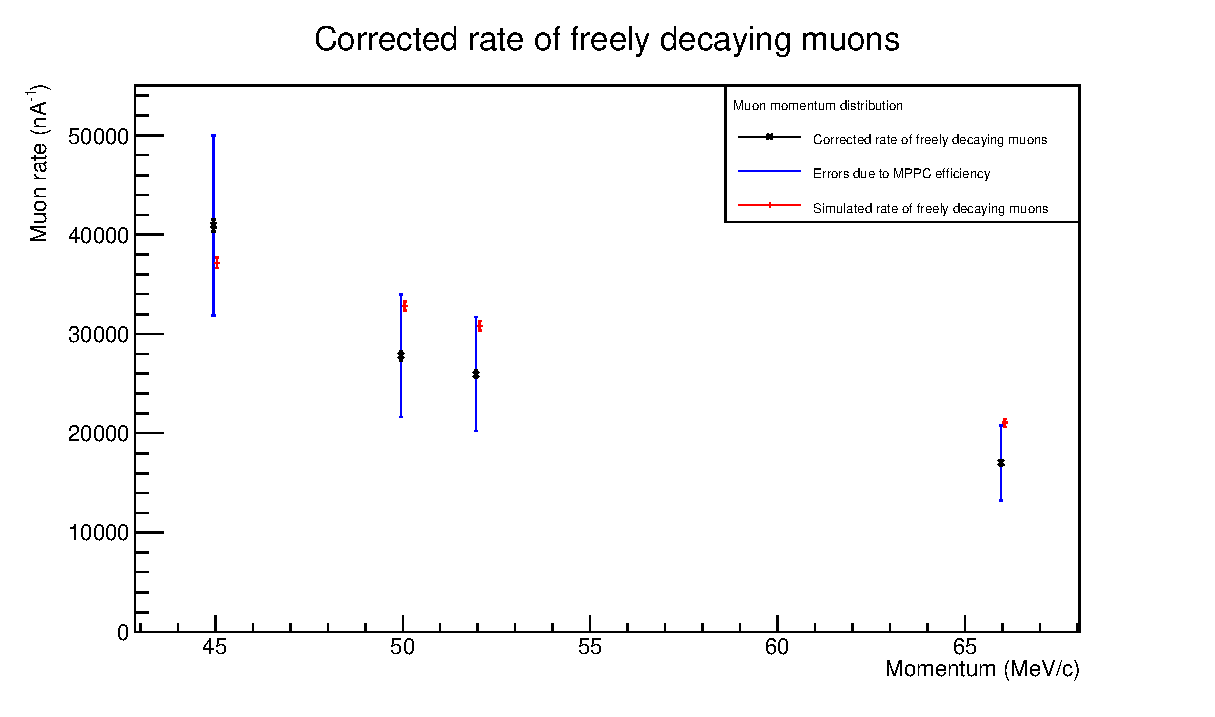
\includegraphics[width=0.8\textwidth]{images/plot_generating_scripts/adjusted_muon_rates.eps}
  \caption{Corrected free muon decay rate and simulated free muon decay rate. The red lines are the simulated results, the blue lines the measured results including the MPPC efficiency error and the black lines are the measured values without the MPPC efficiency error.}
  \label{fig:images_plot_generating_scripts_adjusted_muon_rates}
\end{figure}

\begin{figure}[hptb]
  \centering
    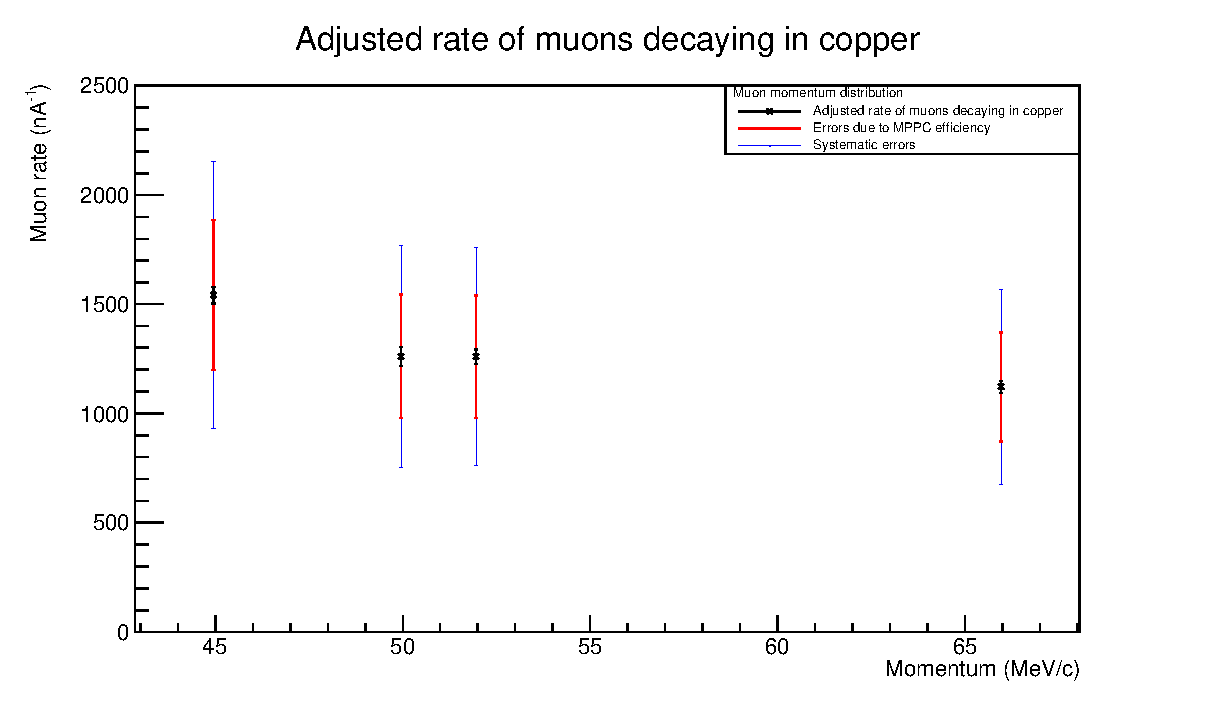
\includegraphics[width=0.8\textwidth]{images/plot_generating_scripts/adjusted_muon_rates_cu.eps}
  \caption{Corrected decay rate of muonic copper. The simulated rates are not shown as the statistics for muonic copper decays were too low to extract reasonable values from. The blue line indicates the error due to systematic error, the red line is the MPPC efficiency error and the black line the statistical error.}
  \label{fig:images_plot_generating_scripts_adjusted_muon_rates_cu}
\end{figure}

\subsection{Analysis} % (fold)
\label{sub:mom_analysis}
As can be seen from figure~\ref{fig:images_plot_generating_scripts_adjusted_muon_rates} there is a good agreement between simulation and experiment. The largest source of errors for this measurement was the lack of accurate information on the detector efficiency and in further measurements this should be corrected. Despite the large errors the data shows a clear reduction in the number of stopped muons as the degrader thickness increases and that this reduction is stable between the repeat measurements. 

Throughout the entire experiment there was a gradual decline in the total trigger rate (even between matched configurations) as is seen in figure~\ref{fig:gain_stability}. The cause of the reduction in trigger rate is unclear, its effect on the results is corrected for through the dead time calculation. 

A point of interest in the data is the difference between the first and subsequent runs. In the first run the simulation predicts a lower rate whilst in all other runs the simulation predicts a higher rate. This suggests that there may be some other effect that needs to be accounted for in either the simulation or the analysis. Another area that needs more accurate modelling is the inclusion of beam effects in order to better understand the sinusoidal noise seen in all data and account for it.

Based on the simulation the stopped muons account for a small portion of the beam, no more than 8~\% of the total muon flux. Using the simulation the fraction of the beam which is stopped for each degrader can be estimated. Using these ratios we can calculate the total muon flux for the RCNP's maximum 1~\(\mu\)A beam:
\begin{align}\label{equ:total_rate}
  T &= 1,000\times\frac{R}{C}
\end{align}
Where \(T\) is the total muon flux per second, \(R\) is the measured muon rate per~nA and \(C\) is the fraction of the beam that was simulated to stop in that configuration. The factor of 1,000 converts from nA to \(\mu\)A and hence to s\(^{-1}\) for a 1~\(\mu\)A proton beam. The calculated values for the total muon flux are shown in table~\ref{tab:total_muon_rates} along with the per~Watt efficiency, using the RCNP's 400~W beam at 1~\(\mu\)A.

\begin{table}
  \lineup
  \begin{center}
  \begin{tabular}{c | r@{\(\pm\)}l | r@{\(\pm\)}l | r@{\(\pm\)}l | r@{\(\pm\)}l}
    Momentum  &  \multicolumn{2}{c|}{Component}
                                  &  \multicolumn{2}{c|}{Rate}
                                                    &  \multicolumn{2}{c|}{Total flux}
                                                                     &  \multicolumn{2}{c}{Efficiency} \\
    (MeV/c)   &  \multicolumn{2}{c|}{(\%)}
                                  &  \multicolumn{2}{c|}{(\(\times10^3\) nA\(^{-1}\))}
                                                    &  \multicolumn{2}{c|}{(\(\times10^8\) s\(^{-1}\))}
                                                                     &  \multicolumn{2}{c}{(\(\times10^5\)~muons~W\(^{-1}\))} \\
    \hline
    448       &  \.8.158 & 0.096  & \042.5 & 13     & \05.21 & 1.62  &   \0\0\013.0 & 4.1  \\
    451       &  \.7.356 & 0.091  & \028.8 & \09.0  & \03.91 & 1.22  &  \0\0\0\09.8 & 3.1  \\
    452       &  \.7.356 & 0.091  & \029.4 & \09.2  & \04.00 & 1.25  &   \0\0\010.0 & 3.1  \\
    455       &  \.6.742 & 0.087  & \027.3 & \08.5  & \04.04 & 1.26  &   \0\0\010.1 & 3.2  \\
    458       &  \.4.665 & 0.071  & \018.0 & \05.6  & \03.86 & 1.20  &  \0\0\0\09.7 & 3.0  \\
    459       &  \.4.665 & 0.071  & \018.4 & \05.7  & \03.94 & 1.23  &  \0\0\0\09.9 & 3.1  \\
  \end{tabular}
  \end{center}
  \caption{Calculated muon production efficiencies and total fluxes at 1~\(\mu\)A. `Component' is the simulated fraction of the total beam that stops in each set up. `Rate' is the sum of the corrected rates for free and copper decays. The total flux was calculated using equation~\eqref{equ:total_rate}. The average total flux is \( (4.16\pm0.92) \times10^8\)~muons~s\(^{-1}\) where the error is the same fractional error as is on the MPPC efficiency, \(\Delta\epsilon_{\textsc{mppc}}^2\sim 22\)~\%. The efficiency is the total flux divided by the full beam power (400~W). The average efficiency of MuSIC is calculated to be \((10.55\pm2.3)\times10^5\)~muons~W\(^{-1}\) which has the same, \(\epsilon_{\textsc{mppc}}^2\) dominated, error as the total flux.}
  \label{tab:total_muon_rates}
\end{table}

Two things are clear from table~\ref{tab:total_muon_rates}: at full power MuSIC should be capable of producing the design goal of \(>10^8\)~muons~s\(^{-1}\) and it should be one of the most intense muon beams in the world. The average intensity, \((4.16\pm0.92)\times10^8\)~muons~s\(^{-1}\), is comparable PSI's most intense muon beam (\(4.8\times10^8\)~muons~s\(^{-1}\)~\cite{mue4_psi}) but achieved with a proton beam significantly less powerful. This last point is best highlighted by comparing the number of muons produced per~Watt of proton beam: PSI produces 292~muons~W\(^{-1}\) whilst MuSIC is predicted to produce \((10.55\pm2.3)\times10^5\)~muons~W\(^{-1}\).

% As has been noted the lack of information on the detector's efficiency was a severe hinderance in the calculation of the muon rate. Further improvements are needed, not only to reduce errors and better understand the detector but to allow testing of the simulation. Work at COMET suggests that there are differences in the particle rates between various simulations (e.g.\ MARS and G4BL), understanding of this will be vital in those measurements.

% subsection mom_analysis (end)


% \chapter{Conclusion} % (fold)
% \label{cha:conclusion}
% %  \(6\times10^8\)~muons/nA)
% Over the course of two years three different measurements of the MuSIC beam-line have been made; each building on the knowledge gathered in the previous. The total charged particle flux was measured and compared to simulation; the muon lifetime was determined and used to confirm their presence; and the number of muon decays under different configurations has been used to determine the momentum flux (as well as the muon flux).
% 
% The three measurements have gone a long way to testing the simulation of MuSIC and to confirming that it is a reasonable approximation to the reality. Further measurements will hopefully refine our knowledge of the beam and maybe begin testing the different models used in the simulation. Work on simulating COMET has already shown that there are differences in the predicted rates of different particles, determining how which simulation is correct will make further work easier and more accurate.
% 
% MuSIC has been shown to perform as expected, producing more muons per proton than any other beam. Even incomplete it's already being used to make new measurements (precisions measurements of decays from muon activated molybdenum) and it is hoped that further funding will help complete this powerful tool. 
% 
% Currently the largest problems with the measurements at MuSIC are in the errors on the measurements but as these are refined more detailed simulations will also be needed. There are two key improvements that can be made to the simulation: larger G4BL run and better digitisation. A larger G4BL run will increase the number of copper stopped muons that will allow detailed investigation of the rates of negative muons stopping in copper, it is also necessary to start making comparisons between different hadron production codes and may provide useful data for refining these at low energy. The second improvement, digitisation, will allow analysis of simulation that's more directly comparable to what's measured. This will be key in understanding backgrounds and having clear understanding of the fine properties of the beam. 
% 

% Over the last three years the simulation of MuSIC has been refined and tuned using data gathered over several periods of beam time. The simulation was written in G4Beamline to cover the bulk portions and Geant4 to test the detectors used. They were also used to compare to the data gathered during the beam-times.
% 
% The three measurements were made over five periods of beam time. Each beam time lasted between 24 and 72 hours. The first measurements were of the charged particle flux, then the muon lifetime was measured and finally the muon momentum distribution was measured. Each measurement was made using simple plastic scintillator detectors with Data Acquisition (DAQ) performed using off the shelf crate systems (NIM, CAMAC and VME). 
% 
% The measurement of the charged particle flux confirmed the beam location to the top and the left of the beam pipe. It also set a benchmark for the particle flux which confirmed the bounds of the maximum muon flux. The measurement determined that the peak particle flux was 90,800\(\pm\)7,000~particles~nA\(^{-1}\) of proton~beam positioned 5~cm above the beam centre (at a distance of 6~cm). The second measurement of the particle flux determined that the beam spot 85~cm from the end of the beam pipe was 25~cm above and 17~cm to the left of the beam centre, with a flux of 10,800\(\pm\)2,100~particles~nA\(^{-1}\). 



% chapter executive_summary (end)

% chapter conclusion (end)